%Mathdocs. This is the master copy, altered on 8/28/2022 for tkzEuclide
\documentclass[addpoints]{amsart} 
%\documentclass{tglat2e}%%   tglat calls the Class of our Journal.
\parskip 5pt
\textwidth 5.5in
\linespread{1.2}
%\hoffset-.2truein
%\vsize10truein
%For large fonts, use \tiny, \scriptsize, \footnotesize, \Large, \LARGE, \huge, \Huge.

\usepackage[hidelinks]{hyperref} %this allows links to appear on the pdf, so you can click them. Then put in \hypersetup{(options for naming the colors of various components)}. To set all colors at once, use allcolors=black. To avoid any sign of links, put in "hidelinks". You can also put in "linktocpage" in the hypersetup, to make it just the page number, not the entire line in the table of contents. This is in StackExchange on "how can I make a clickable table of contents?"
\hypersetup{allcolors=black}

\usepackage{gensymb} %for degree symbol
\usepackage{pgf, tikz} %8/26/22 I put in the pgf for Euclide
%\usepackage{tikzsymbols} %for emoticons! Call with \Smiley, \Sadey, \Neutrey, and put [2.0] to make it twice as big. see lists.
\usepackage{tikz-cd} %Commutative Diagrams. Use \[\begin{tikzcd} .. \end{tikzcd}\] You can make: A \arrow[hook]{r} & B
\usetikzlibrary{angles,arrows.meta,automata,backgrounds,calc,decorations.markings,decorations.pathreplacing,intersections,patterns,positioning,quotes} %For background figures, use \begin{scope}[on background layer] ... \end{scope}
\usetikzlibrary{shapes} %For polygon nodes, see http://www.texample.net/tikz/examples/node-shapes/
\usepgflibrary{shapes.geometric}
\usepackage{tkz-euclide} 
%Needed to resolve conflict between tkz-euclide and thmtools, see https://tex.stackexchange.com/questions/456029/thmtools-and-tkz-euclide-conflict
%\usetkzobj{all}
%\usepackage{thmtools}
\usepackage{etoolbox}
\usepackage{placeins}

\usepackage{mdframed} %\begin{mdframed}[backgroundcolor=green!10,linewidth=1pt] makes a colored box around an enumerate, etc.
\usepackage{pgfplots}
\pgfplotsset{width=10cm,compat=1.9}
\usepackage[export]{adjustbox}
\usepackage{caption}
\usepackage{subcaption}
\usepackage{wrapfig}
%See sharelatex.com
\usepackage{graphicx}
\usepackage{mathtools}  %This allows the \begin{bmatrix*} environment, and a [r] [l], or [c] which aligns the entries!
%See sharelatex.com
\usepackage{amsthm,thmtools} %This allows boxed theorem-like environments, see \declaretheorem as below
%I removed this 8/26/2022 trying to fix euclide, as I heard there was a conflict.
\usepackage{relsize} %for a cup product $\mathsmaller\cup$


\usepackage{amsmath,systeme} %this is for systems of equations. 
%You use \begin{equation*}\systeme{<put in system, separating equations with a comma>}\end{equation*}. 
%If you want to get rid of the delimiter, use \sysdelim..\systeme{ } instead.

\usepackage{fancyhdr} %headers and footers. On the document, put \pagestyle{fancy} before begin{document}, then use \rhead{Cal Poly}, \chead{\bf Math 241}, \lhead{Brussel}. Or, \fancyhead[L]{Math 483/560}, \fancyhead[R]{Brussel}, \fancyhead[C]{Structure}, then \begin{document}\thispagestyle{fancy} <- If you want the first page as well.

%FONTS: On 10/21/2023 I blocked Asher's mathrsfs, in favor of mathalfa.
\usepackage{fdsymbol} %Or {mnsymbol} This is for the math font in regular use.
%%\usepackage{amssymb, latexsym, amsmath} %is what we had before fdsymbol%, makeidx}
%%\makeindex
\usepackage{courier}
%call it up with \texttt.  It gives an equally spaced courier font.
\usepackage[scr=rsfso]{mathalfa} %If I put this on the document itself it works, otherwise no.
\input ArtNouvc.fd
\newcommand*\initfamily{\usefont{U}{ArtNouvc}{xl}{n}} %Fancy all caps. Call it with {\initfamily <text>}
\input Starburst.fd
\newcommand*\starinitfamily{\usefont{U}{Starburst}{xl}{n}}

\usepackage[all,cmtip]{xy}
%See website http://en.wikibooks.org/wiki/LaTeX/Creating_Graphics#XY-pic
%http://www.tug.org/pracjourn/2006-4/blaga/blaga.pdf

\usepackage{enumerate}
%Follow the usual \begin{enumerate} with [I] for roman numerals, and [(a)] for alphabetic symbols.
\usepackage{multicol} %Put \begin{multicol}{2} for two columns of enumerate. Place before \begin{enumerate}, and then \end{multicol} after.
\usepackage{mdwlist}

%I blocked this when I put in tikz, because of a color clash.
%\usepackage[usenames, dvipsnames]{color}
%See website http://people.oregonstate.edu/~peterseb/tex/samples/color-package.html for
%a list of the many color options.  Or, http://en.wikibooks.org/wiki/LaTeX/Colors
%To invoke, use {\color{red}<text>}
%To make a new color, use \definecolor{orange}{rgb}{1,0.5,0}  Here rgb is red green blue.

%\usepackage{mathrsfs} %nice script font
%%% UV - changes in header: %'d \usepackage{mathabx}, \def\divides, \def\notdivides.
%\usepackage{mathabx} % get \notdivides

\usepackage[OT2,T1]{fontenc}
\DeclareSymbolFont{cyrletters}{OT2}{wncyr}{m}{n}
\DeclareMathSymbol{\Sha}{\mathalpha}{cyrletters}{"58}



\theoremstyle{plain}
\newtheorem{Theorem}[subsection]{Theorem}
\newtheorem{Lemma}[subsection]{Lemma}
\newtheorem{Corollary}[subsection]{Corollary}
\newtheorem{Proposition}[subsection]{Proposition}
\newtheorem{Notation}[subsection]{Notation}
\newtheorem{Definition}[subsection]{Definition}
%\newtheorem{Equation}[subsection]{Equation}
%the [equation] makes sure the numbering is coherent.
%Can put [subsubsection]  in to line up with subsubsection numbering. With Equation this doesn't seem to be right.

%\theoremstyle{definition} %Doesn't seem to matter.
\theoremstyle{remark}%This doesn't seem to work.
\newtheorem{Example}[subsubsection]{\bf Example}
\newtheorem{Examples}[subsubsection]{\bf Examples}
\newtheorem{Problem}[subsubsection]{Problem}
\newtheorem{Paragraph}[subsubsection]{}
\newtheorem{Remark}[subsubsection]{\bf Remark}
\newtheorem{Remarks}[subsubsection]{\bf Remarks}
\numberwithin{equation}{subsection}

%For undergraduate docs, these are more fun ways to box theorems and definitions, and order examples and exercises.
%Blue:\declaretheorem[shaded={rulecolor={rgb}{0,0,1},rulewidth=1pt, bgcolor={rgb}{0.95,0.95,1}},name={\bf Theorem}]{thm}
%Red: \declaretheorem[numberlike=thm,shaded={rulecolor={rgb}{1,0,0}, rulewidth=1pt, bgcolor={rgb}{1,0.95,0.95}},name={\bf Definition}]{defn}
\declaretheorem[shaded={rulecolor={rgb}{0,0,0},rulewidth=1pt, bgcolor={RGB}{255, 255, 255}},name={\bf Theorem}]{thm}\declaretheorem[numberlike=thm,shaded={rulecolor={rgb}{0,0,0}, rulewidth=1pt, bgcolor={RGB}{255, 255, 255}},name={\bf Definition}]{defn}\declaretheorem[numberlike=thm,name={\bf Example}]{ex}
\declaretheorem[numberlike=thm,name={\bf Exercise}]{exer}
\declaretheorem[numberlike=thm,shaded={rulecolor={rgb}{0,0,0}, rulewidth=1pt, bgcolor={RGB}{255, 255, 255}},name={\bf Lemma}]{lma}
\declaretheorem[numberlike=thm,shaded={rulecolor={rgb}{0,0,0}, rulewidth=1pt, bgcolor={RGB}{255, 255, 255}},name={\bf Proposition}]{prop}
\declaretheorem[numberlike=thm,shaded={rulecolor={rgb}{0,0,0}, rulewidth=1pt, bgcolor={RGB}{255, 255, 255}},name={\bf Corollary}]{corly}

%%   NEW! This is an example of a new environment. It resembles
%% theorem-like environments in usage and definition.
%% You type \newdefinition{<def_name>}{<Definition>} in a preamble
%% or in your own style file and then use automatically numbering
%% environment <def_name> for `<Definition> NN' in text.
%% \newexample is equal to \newdefinition since they
%% produce identical environments. Use whatever you like.
%%   We included some common definitions for convenient typesetting.
%% You can use the following environments:
%%  definition for Definition 57.
%%  example for Example 57.
%%  theorem for Theorem 57.
%%  lemma for Lemma 57.



%%   NEW! No-numbered environments `remark' and `demo' invented.
%% Used with optional argument they produce it in a suitable way.
%% If no they produce standard `Remark.' and `Proof.' text.
%% Be careful not to use [ right after \begin{remark/demo} ---
%% or protect it stating an empty group in the following way: {}[.



%% Do NOT redefine one- and two-character LaTeX commands
%% (like "\r", "\O", "\L", "\AA", etc.)!

%\newcommand{\e}{{\varepsilon}}

%Script commands:
\newcommand{\bb}[1]{{\bold{#1}}}
\newcommand{\bs}[1]{{\boldsymbol{#1}}}
\newcommand{\scr}[1]{{\mathscr{#1}}}
\newcommand{\cat}[1]{{\sf{#1}}}
\newcommand{\mbb}[1]{{\mathbb{#1}}}
\newcommand{\mc}[1]{{\mathcal{#1}}}
\newcommand{\mf}[1]{{\mathfrak{#1}}}
\newcommand\ssf[1]{{\sf{#1}}}

%Normal lower case letters
\renewcommand{\a}{{\bs a}}
\renewcommand{\b}{{\bs b}}
\renewcommand{\c}{{\bs c}}
\newcommand{\ba}{{\bb a}}
\newcommand{\bc}{{\bb c}}
\newcommand{\bB}{{\bb B}}
\newcommand{\bN}{{\bb N}}
\newcommand{\bT}{{\bb T}}
\newcommand\bU{{\bb U}}
\newcommand\bsa{{\bs a}}
\newcommand\bsb{{\bs b}}
\newcommand\bsc{{\bs c}}
\newcommand\bsB{{\bs B}}
\newcommand\bsN{{\bs N}}
\newcommand\bsT{{\bs T}}
\newcommand\bsU{{\bs U}}
%\newcommand{\c}{{\bold c}}
\newcommand{\e}{{\bold e}}
\newcommand{\f}{{\bold f}}
\newcommand{\g}{{\mathsf g}}
\newcommand{\h}{{\text{\rm h}}}
\newcommand{\ch}{{\text{\rm h}}} %in case we redefine \h to mean \bold h.
\renewcommand{\i}{{\boldsymbol i}}
\renewcommand{\j}{{\boldsymbol j}}
\renewcommand{\k}{{\boldsymbol k}}
%\renewcommand{\k}{{\kappa}}
\newcommand{\m}{{\frak m}}
\newcommand{\n}{{\bold n}}
\renewcommand{\o}{{\text{\rm o}}}
\newcommand{\p}{{\frak p}}
\newcommand{\q}{{\frak q}}
\renewcommand{\r}{{\bold r}}
\newcommand{\s}{{\text{\rm s}}}
\renewcommand\u{{\boldsymbol u}}
\renewcommand\v{{\boldsymbol v}}
\newcommand\w{{\boldsymbol w}}
\newcommand\x{{\bold x}}
\newcommand\y{{\bold y}}
\newcommand\z{{\bold z}}

\newcommand\0{{\boldsymbol 0}}
\renewcommand\1{{\boldsymbol 1}}

\newcommand{\A}{{\mathbb A}}
\newcommand{\Ac}{{\text{\rm A}}}
%\newcommand{\B}{{\mathbb B}}
\newcommand{\B}{{\text{\rm B}}}
\newcommand{\cB}{{\text{\rm B}}}
\newcommand{\C}{{\mathbb C}}
\newcommand{\CC}{{\mathscr C}}
\newcommand{\Dg}{{\text{\rm D}}}
\newcommand{\DD}{{\mathfrak D}}
\newcommand{\E}{{\mathscr E}}
\newcommand{\EE}{{\mathfrak E}}
\newcommand{\Eu}{{\mathbb E}}
\newcommand{\F}{{\mathbb F}}
\newcommand{\FF}{{\scr{F}}}
\newcommand{\G}{{\mathsf G}}
\newcommand{\Ga}{{\text{\rm G}_{\text{\rm a}}}}
\newcommand{\GG}{{\scr{G}}}
\newcommand{\Gm}{{\text{\rm G}_{\text{\rm m}}}}
%\renewcommand{\H}{{\text{\rm H}}}
\newcommand{\cH}{{\text{\rm H}}}
\renewcommand{\H}{{\mathbb H}}
\newcommand{\HH}{{\scr{H}}}
\newcommand{\I}{{\mathrm{I}}}
\newcommand{\Is}{{\text{\rm I}}}
\newcommand{\J}{{\mathscr J}}
\newcommand{\K}{{\text{\rm K}}}
\renewcommand{\L}{{\mathscr L}}
\newcommand{\cL}{{\text{\rm L}}}
\newcommand{\nL}{{{}_n\text{\rm L}}}
\newcommand{\M}{{\text{\rm M}}}
\newcommand{\MM}{{\mathfrak M}}
\newcommand{\N}{{\mathbb N}}
\renewcommand{\O}{{\mathsf{O}}}
\newcommand{\Nm}{{\text{\rm N}}}
\newcommand{\Nrd}{{\text{\rm Nrd}}}
\newcommand{\Nrm}{{\mathcal N}}
\newcommand{\NS}{{\text{\rm NS}}}
\renewcommand{\P}{{\mathbb P}}
\newcommand{\Q}{{\mathbb Q}}
\newcommand{\cR}{{\text{\rm R}}}
\newcommand{\R}{{\mathbb R}}
\newcommand{\Rt}{{\text{\rm R}}}
\renewcommand{\S}{{\mathsf{S}}}
%\newcommand{\T}{{\mathcal S_Y}}
\newcommand{\T}{{\mathsf{T}}}
\newcommand{\Tr}{{\text{\rm Tr}}}
\newcommand{\TF}{{\text{\rm TF}}}
\newcommand{\TT}{{\mathfrak{T}}}
%\renewcommand{\U}{{\Cal S_Z}}
\renewcommand{\U}{{\mathsf{U}}}
\newcommand{\UC}{{\text{\rm C}}}
\newcommand{\UD}{{\text{\rm UD}}}
\newcommand{\UR}{{\text{\rm R}}}
\newcommand{\UZ}{{\text{\rm Z}}}
\newcommand{\UZn}{{\text{\rm U$\Z_n^N$}}}
\newcommand{\V}{{\mathsf V}}
\newcommand{\W}{{\text{\rm W}}}
\newcommand{\X}{{\text{\rm X}}}
\newcommand{\Y}{{\mathbb Y}}
\newcommand{\Z}{{\mathbb Z}}
\newcommand{\cZ}{{\text{\rm Z}}}


\newcommand{\ab}{{\text{\rm ab}}}
\newcommand{\ad}{{\text{\rm ad}}}
\newcommand{\adj}{{\text{\rm adj}}}
\newcommand{\alg}{{\text{\rm alg}}}
\newcommand{\alt}{{\text{\rm alt}}}
\newcommand{\ave}{{\text{\rm ave}}}
\newcommand{\avg}{{\text{\rm avg}}}
\newcommand{\bit}[1]{{\textbf{\textit{#1}}}}
\newcommand{\blue}[1]{{\color{blue}{#1}}}
\newcommand{\bmx}[1]{{\begin{bmatrix}#1\end{bmatrix}}}
\newcommand{\bmxr}[1]{{\begin{bmatrix*}[r]#1\end{bmatrix*}}}
\newcommand{\sbmx}[1]{{\left[\begin{smallmatrix}#1\end{smallmatrix}\right]}}
\newcommand{\sbmxr}[1]{{\left[\begin{smallmatrix*}[r]#1\end{smallmatrix*}\right]}}
\newcommand{\sdbmx}[1]{{\text{\footnotesize $\begin{bmatrix}#1\end{bmatrix}$}}} %smaller for display
\newcommand{\sdbmxr}[1]{{\text{\footnotesize $\begin{bmatrix*}[r]#1\end{bmatrix*}$}}} %smaller for display
\newcommand{\mx}[4]{{\text{\footnotesize $\begin{bmatrix}#1&#2\\#3&#4\end{bmatrix}$}}} %smaller for display
\newcommand{\pmx}[1]{{\begin{pmatrix}#1\end{pmatrix}}}
\newcommand{\vmx}[1]{{\begin{vmatrix}#1\end{vmatrix}}}
\newcommand{\vmxr}[1]{{\begin{vmatrix*}[r]#1\end{vmatrix*}}}
\newcommand{\sdvmxr}[1]{{\text{\footnotesize $\begin{vmatrix*}[r]#1\end{vmatrix*}$}}} %smaller for display
\newcommand{\sdvmx}[1]{{\text{\footnotesize $\begin{vmatrix*}#1\end{vmatrix*}$}}} %smaller for display
\newcommand{\svmxr}[1]{{\left|\begin{smallmatrix*}[r]#1\end{smallmatrix*}\right|}} %smaller
\newcommand{\Vmx}[1]{{\begin{Vmatrix}#1\end{Vmatrix}}} %double absolute value
\newcommand{\br}[1]{{\langle{#1}\rangle}}
\newcommand{\bbr}[1]{{\big\langle{#1}\big\rangle}}
\newcommand{\bbbr}[1]{{\left<{#1}\right>}}
\newcommand{\bull}{{\noindent $\bullet\;$}}
\newcommand{\cd}{{\text{\rm cd}}}
\newcommand{\car}{{\text{\rm char}}}
\newcommand{\chr}{\mathrm{char}}
\newcommand{\codim}{{\text{\rm codim}}}
\newcommand{\coker}{{\text{\rm coker}}}
\newcommand{\cok}{{\text{\rm cok}}}
\newcommand{\col}{{\mathsf{col}}}
\newcommand{\cor}{{\text{\rm cor}}}
\newcommand{\comp}{{\text{\rm comp}}}
\newcommand{\cont}{{\text{\rm cont}}}
\newcommand{\cs}{{\text{\rm cs}}}
\newcommand{\dd}[1]{{\frac{d}{d#1}}}
\newcommand{\sdd}[1]{{\text{\footnotesize $\frac{d}{d#1}$}}}
\newcommand{\ddd}[2]{{\frac{d#1}{d#2}}}
\newcommand{\sddd}[2]{{\frac{\text{\footnotesize$d#1$}}{\text{\footnotesize$d#2$}}}}
%\newcommand{\sddd}[2]{{\text{\footnotesize $\frac{d#1}{d#2}$}}}
\renewcommand{\det}{{\text{\rm det}}}
\newcommand{\df}{{\,\overset{\text{\rm df}}{=}\,}}
\newcommand{\diag}{{\text{\rm diag}}}
\newcommand{\disc}{{\text{\rm disc}}}
\newcommand{\dR}{{\text{\rm dR}}}
\newcommand{\ds}[1]{{\displaystyle{#1}}}
\renewcommand{\div}{{\text{\rm div}}}
\renewcommand{\dim}{{\text{\rm dim\,}}}
\newcommand{\edge}[1]{{\overline{#1}}}
%\renewcommand{\endpf}{{\hfill $\blacksquare$}}
\renewcommand{\exp}{{\mathsf{exp}}}
\newcommand{\ep}{{\varepsilon}}
\newcommand{\et}{{\text{\rm \'et}}}
\renewcommand{\gcd}{{\text{\rm gcd}}}
\newcommand{\gl}{{\mathsf{gl}}}
\newcommand{\gldim}{{\text{\rm glob\,dim}\,}}
\newcommand{\good}{{\text{\rm good}}}
\newcommand{\gr}{{\text{\rm gr}}}
\newcommand{\grad}{{\boldsymbol{\triangledown}\!}}
\newcommand{\height}{{\text{\rm ht}\,}}
\newcommand{\id}{{\text{\rm id}}}
\newcommand{\im}{{\text{\rm im}}}
\newcommand{\ind}{{\text{\rm ind}}}
\renewcommand{\inf}{{\text{\rm inf}\,}}
\newcommand{\init}{{\text{\rm init}}}
\newcommand{\inv}{{\text{\rm inv}}}
\newcommand{\isim}{{\;\overset{\sim}{\longrightarrow}\;}}
\newcommand{\isom}{{\;\simeq\;}}
\newcommand{\kalg}{{k\text{\rm -alg}}}
\renewcommand{\ker}{{\text{\rm ker}}}
\newcommand\kup{{\,\Small{\cup}\,}}
\newcommand{\lcm}{{\text{\rm lcm}}}
\newcommand{\length}{{\text{\rm length}}}
\renewcommand{\ll}{\longleftarrow}
\newcommand{\lm}{\longmapsto}
\newcommand{\lr}{\longrightarrow}
\newcommand\dashlr{\,\tikz[baseline]{\draw[dashed, ->, -latex] (0,.1)--(.55,.1);}\;}
\newcommand{\mer}{{\text{\rm mer}}}
\newcommand{\mmu}{{\mbox{\boldmath $\mu$}}}
\newcommand{\mult}{{{\sf mult}}}
\newcommand{\mywedge}[1]{{\bigwedge}^{\kern-1pt{#1}}}
\newcommand{\ndiv}{{\,\not\big |\,}}
\newcommand{\normal}{{\triangleleft\;}}
\newcommand{\nr}{{\text{\rm nr}}}
\newcommand{\ns}{{\text{\rm ns}}}
\newcommand{\ob}[1]{{\,\overline{\!#1}}}
\newcommand{\ol}[1]{{\overline{#1}}}
\newcommand{\olra}[1]{{\overleftrightarrow{#1}}}
\newcommand{\on}{{\mathsf{o}_n}}
\newcommand{\onto}{{\,\twoheadrightarrow\,}}
\newcommand{\op}{{\sf{op}}}
\newcommand{\ora}[1]{{\overrightarrow{#1}}}
\newcommand{\orb}{{\text{\rm orb}}}
\newcommand{\orbit}{{\text{\rm orbit}}}
\newcommand{\ord}{{\sf{ord}}}
%\newcommand{\overbar}[1]{\mkern 1.5mu\overline{\mkern-1.5mu#1\mkern-1.5mu}\mkern 1.5mu}
\newcommand{\overbar}[1]{{\,\overline{\!#1}}}
\newcommand{\pdd}[1]{{\frac{\partial}{\partial#1}}}
\newcommand{\spdd}[1]{{\text{\footnotesize $\frac{\partial}{\partial#1}$}}}
\newcommand{\tpdd}[1]{{\text{\tiny $\frac{\partial}{\partial#1}$}}}
\newcommand{\ppd}[2]{{\frac{\partial#1}{\partial#2}}}
\newcommand{\sppd}[2]{{\frac{\text{\footnotesize$\partial#1$}}{\text{\footnotesize$\partial#2$}}}}
%\newcommand{\sppd}[2]{{\text{\footnotesize $\frac{\partial#1}{\partial#2}$}}}
\newcommand{\per}{{\text{\rm per}}}
\newcommand{\pf}{{\noindent{\it Proof.}\;\;}}
\newcommand{\pos}{{\text{\rm pos}}}
\renewcommand{\pmod}[1]{{\text{\rm (mod ${#1}$)}}}
\newcommand{\prestar}{{{}^*\!}}
\newcommand{\prob}[1]{{\noindent{\bf{#1}}}}
\newcommand{\pfaff}{{\text{\rm pfaff}}}
\newcommand{\proj}{{\mathsf{proj}}}
\newcommand{\rad}{{\text{\rm rad}}}
\newcommand{\ram}{{\text{\rm ram}}}
\newcommand{\ramloc}{{\text{\rm ram.loc.}}}
\newcommand{\rdim}{\mathrm{rdim}}
\newcommand{\red}{{\text{\rm red}}}
\newcommand{\reg}{{\text{\rm reg}}}
\newcommand{\res}{{\text{\rm res}}}
\newcommand{\rk}{{\text{\rm rk}}}
\newcommand{\row}{{\mathsf{row}}}
\newcommand{\rref}{{\mathsf{rref}}}
\newcommand{\scd}{{\text{\rm scd}}}
\newcommand{\sep}{{\text{\rm sep}}}
\newcommand\sech{{\text{\rm sech}}}
\newcommand{\sfrac}[2]{{\frac{\text{\footnotesize$#1$}}{\text{\footnotesize$#2$}}}}
\newcommand{\sgn}{{\text{\rm sgn}}}
\newcommand{\sh}{{\text{\rm sh}}}
\newcommand{\sign}{{\text{\rm sign}}}
\renewcommand{\skew}{{\mathsf{skew}}}
\newcommand{\so}{{\mathsf{so}}}
\newcommand{\su}{{\mathsf{su}}}
\renewcommand{\sp}{{\mathsf{sp}}}
\newcommand{\spn}{{\text{\rm span}}}
\newcommand{\spec}{{\text{\rm Spec}}}
\newcommand{\stab}{{\sf{stab}}}
\newcommand{\supp}{{\text{\rm supp}}}
\newcommand{\tor}{{\text{\rm tor}}}
\newcommand{\tr}{{\text{\rm t}}}
\newcommand{\trdeg}{\mathrm{trdeg}}
\newcommand{\tri}{{\triangle}}
\newcommand{\tworight}{{\;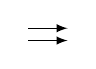
\begin{tikzpicture}\draw[->,-latex](0,5/32)--(1/2,5/32);\draw[->,-latex](0,0)--(1/2,0);\end{tikzpicture}\;}}
\newcommand{\trix}{\noindent$\hphantom{\quad}*\;$}
\newcommand{\ul}[1]{{\underline{#1}}}
\newcommand{\un}[1]{{\underline{#1}}}
\newcommand{\vnr}{{\text{\rm $v$-nr}}}
\newcommand\wh[1]{{\widehat{#1}}}
\newcommand{\widesim}[1][1.5]{\mathrel{{\scalebox{#1}[1]{$\sim$}}}} %to use this, type \widesym for a 1.5x \sim, and type \widesim[2] to make it 2x original size.
\newcommand\wt[1]{{\widetilde{#1}}}
\newcommand{\zar}{{\text{\rm Zar}}}



\newcommand{\Ad}{{\text{\rm Ad}}}
\newcommand{\Alb}{{\text{\rm Alb}}}
\newcommand{\Alt}{{\text{\rm Alt}}}
\newcommand{\Ann}{{\mathsf{Ann}}}
\newcommand{\Arc}{{\sf{Arc}}}
\newcommand{\Arccos}{{\text{\rm Arccos}}}
\newcommand{\Arccot}{{\text{\rm Arccot}}}
\newcommand{\Arcsin}{{\text{\rm Arcsin}}}
\newcommand{\Arctan}{{\text{\rm Arctan}}}
\newcommand{\Arg}{{\sf{Arg}}}
\newcommand{\Ass}{{\mathsf{Ass}}}
\newcommand{\ATors}{\text{\rm $A$-Tors}}
\newcommand{\Aut}{{\mathsf{Aut}}}
\newcommand{\Bil}{{\text{\rm Bil}}}
\newcommand{\Bl}{{\text{\rm Bl}}}
\newcommand{\Br}{{\text{\rm Br}}}
\newcommand{\Brdim}{{\text{\rm Br.dim}}}
\newcommand{\nBrdim}{{{}_n\text{\rm Br.dim}}}
\newcommand{\CaCl}{{\text{\rm CaCl}\,}}
\newcommand{\Card}{{\text{\rm Card}}}
\newcommand{\Cl}{{\text{\rm Cl}}}
\newcommand{\CH}{{\text{\rm CH}}}
\newcommand{\Cong}{{\text{\rm Cong}}}
\newcommand{\CSA}{\text{\rm CSA}}
\newcommand{\Ddim}{{\text{\rm D.dim}}}
\newcommand{\Dd}{{\text{\rm Dd}}}
\newcommand{\Der}{{\text{\rm Der}}}
\newcommand{\Div}{{\text{\rm Div}}}
\newcommand{\End}{{\text{\rm End}}}
\newcommand{\Euc}{{\mathsf{Euc}}}
\newcommand{\Exp}{{\text{\rm Exp}}}
\newcommand{\Ext}{{\text{\rm Ext}}}
\newcommand{\Fam}{\mathsf{Fam}}
\newcommand{\Frac}{{\text{\rm Frac}\,}}
\newcommand{\Gal}{{\text{\rm Gal}}}
\newcommand{\GGal}{{\text{\rm $G$-Gal}}}
\newcommand{\GL}{{\mathsf{GL}}}
\newcommand{\Gr}{{\mathsf{Gr}}}
\newcommand{\Grass}{{\text{\rm Grass}}}
\newcommand{\Hom}{{\text{\rm Hom}}}
\newcommand{\Homloc}{{\text{\rm Hom.loc}}}
\newcommand{\II}{{\Cal I\!\Cal I}}
\renewcommand{\Im}{{\text{\rm Im}}}
\newcommand{\Inn}{{\mathsf{Inn}}}
\newcommand{\Isom}{{\mathsf{Isom}}}
\newcommand{\Jac}{{\text{\rm Jac}}}
\newcommand{\JCF}{{\text{\rm JCF}}}
\newcommand{\Length}{{\text{\rm L}}}
\newcommand{\Lin}{{\text{\rm Lin}}}
\newcommand{\Log}{{\text{\rm Log}}}
\newcommand{\Norm}{{\text{\rm N}}}
\newcommand{\Ob}{{\mathsf{Ob}}}
\newcommand{\Of}{{\text{\rm Of}}}
\newcommand{\Out}{{\text{\rm Out}}}
\newcommand{\Pf}{{\noindent{\it Proof.}\;\;}}
\newcommand{\PGL}{{\mathsf{PGL}}}
\newcommand{\Pic}{{\text{\rm Pic\,}}}
\newcommand{\Princ}{{\text{\rm Princ}\,}}
\newcommand{\Proj}{{\text{\rm Proj}\,}}
\newcommand{\PSL}{{\mathsf{PSL}}}
\newcommand{\PSO}{{\mathsf{PSO}}}
\newcommand{\RCF}{{\text{\rm RCF}}}
\renewcommand{\Re}{{\text{\rm Re}}}
\newcommand{\Rev}{{\text{\rm Rev}}}
\newcommand{\Res}{{\mathsf{Res}}}
\newcommand{\SB}{{\text{\rm SB}}}
\newcommand{\SBV}{{\text{\rm SBV}}}
\newcommand{\Sim}{{\mathsf{Sim}}}
\newcommand{\SK}{{\text{\rm SK}}}
\newcommand{\Skew}{{\mathsf{Skew}}}
\newcommand{\SL}{{\mathsf{SL}}}
\newcommand{\SNF}{{\mathsf{SNF}}}
\newcommand{\SU}{{\mathsf{SU}}}
\newcommand{\SO}{{\mathsf{SO}}}
\newcommand{\Sp}{{\mathsf{Sp}}}
\newcommand{\Spin}{{\mathsf{Spin}}}
\newcommand{\Span}{{\mathsf{Span}}}
\newcommand{\Supp}{{\mathsf{Supp}}}
\newcommand{\Spec}{{\mathsf{Spec}\,}}
\newcommand{\Sym}{{\text{\rm Sym}\,}}
\newcommand\Tan{{\text{\rm Tan}}}
\newcommand{\Tor}{{\text{\rm Tor}}}
\newcommand{\Vol}{{\text{\rm Vol}}}
\newcommand{\Zar}{{\text{\rm Zar}}}

%categories
\newcommand{\Ab}{{\mathsf{Ab}}}
\newcommand{\AbGp}{{\mathsf{AbGp}}}
\newcommand{\AffSch}{{\mathsf{Aff.Sch}}}
\newcommand{\affsch}{{\mathsf{aff.sch}}}
\newcommand{\falg}[1]{{\mathsf{#1}\text{-}\mathsf{alg}}}
\newcommand{\fgAlg}[1]{{\mathsf{f.g.}\mathsf{#1}\text{-}\mathsf{Alg}}}
\newcommand{\Alg}[1]{{\mathsf{#1}\text{-}\mathsf{Alg}}}
\newcommand{\Cat}{\mathsf{Cat}}
\newcommand{\CommRing}{{\mathsf{CommRing}}}
\newcommand{\FibCat}{\mathsf{Fib.Cat}}
\newcommand{\Field}{\mathsf{Field}}
\newcommand{\Fun}{\mathsf{Fun}}
\newcommand{\Grp}{\mathsf{Grp}}
\newcommand{\GSet}{\mathsf{G}\text{-}\mathsf{Set}}
\newcommand{\LRSpaces}{\mathsf{L.R.Spaces}}
\newcommand{\kAff}{{\mathsf{k}\text{-}\mathsf{Aff}}}
\newcommand{\kAlg}{{\mathsf{k}\text{-}\mathsf{Alg}}}
\newcommand{\kAffAlg}{{\mathsf{k}\text{-}\mathsf{AffAlg}}}
\newcommand{\kprimeAlg}{{\mathsf{k'}\text{-}\mathsf{Alg}}}
\newcommand{\kSpec}{{\mathsf{k}\text{-}\mathsf{Spec}}}
\newcommand{\kVar}{\mathsf{k}\text{-}\mathsf{Var}}
\newcommand{\kVec}{\mathsf{k}\text{-}\mathsf{Vec}}
\newcommand{\KVec}{\mathsf{K}\text{-}\mathsf{Vec}}
\newcommand{\Mod}[1]{{\mathsf{#1}\text{-}\mathsf{Mod}}}
\newcommand{\Mor}{{\mathsf{Mor}}}
\newcommand{\Presheaves}{\mathsf{Presheaves}}
\newcommand{\PVar}{\text{$P$\text{-}$\mathsf{Var}$}}
\newcommand{\ProjSch}{{\mathsf{Proj.Sch}}}
\newcommand{\QCoh}{{\mathsf{Q.Coh}}}
\newcommand{\QProjSch}{{\mathsf{Q.Proj.Sch}}}
\newcommand{\Ring}{{\mathsf{Ring}}}
\newcommand{\Sch}{{\mathsf{Sch}}}
\newcommand{\SepPresheaves}{\mathsf{Sep.Presheaves}}
\newcommand{\Set}{\mathsf{Set}}
\newcommand{\Sheaves}{\mathsf{Sheaves}}
\newcommand{\Stacks}{\mathsf{Stack}}
\newcommand{\Top}{\mathsf{Top}}
\newcommand{\Var}[1]{\mathsf{#1}\text{-}\mathsf{Var}}
\renewcommand{\Vec}{{\mathsf{Vec}}}


\newcommand{\BBr}{\mathrm{Br}}
\newcommand{\CPAlg}{\mathrm{CPAlg}}
%\newcommand{\Gal}{\mathrm{Gal}}
\newcommand{\GGL}{\mathrm{GL}}
%\newcommand{\Hom}{\mathrm{Hom}}
\newcommand{\Mat}{\mathrm{M}}
\newcommand{\PPI}{\mathrm{Br.dim}}
%\newcommand{\PGL}{\mathrm{PGL}}
%\newcommand{\GL}{\mathrm{GL}}
%\newcommand{\PSL}{\mathrm{PSL}}
\newcommand{\SSL}{\mathrm{SL}}
\newcommand{\Trd}{\mathrm{Trd}}

% \DeclareMathOperator{\chr}{char}
% \DeclareMathOperator{\charac}{char}
% \DeclareMathOperator{\ind}{ind}
% \DeclareMathOperator{\per}{per}
% \DeclareMathOperator{\res}{res}
% \DeclareMathOperator{\rdim}{rdim}
% \DeclareMathOperator{\trdeg}{trdeg}

% \DeclareMathOperator{\BBr}{Br}
% \DeclareMathOperator{\CPAlg}{CPAlg}
% \DeclareMathOperator{\Gal}{Gal}
% \DeclareMathOperator{\GGL}{GL}
% \DeclareMathOperator{\Hom}{Hom}
% \DeclareMathOperator{\Mat}{M}
% \DeclareMathOperator{\PPI}{Br.\!dim}
% \DeclareMathOperator{\PGL}{PGL}
% \DeclareMathOperator{\PSL}{PSL}
% \DeclareMathOperator{\SSL}{SL}
%\DeclareMathOperator{\Spec}{Spec}
% \DeclareMathOperator{\Spin}{Spin}
% \DeclareMathOperator{\SSK}{SK}
% \DeclareMathOperator{\Trd}{Trd}


%%%%%%%%%%%%%%%

\usepackage{tikz-3dplot}


\renewcommand{\S}{{\mathsf{S}}}
\renewcommand{\T}{{\mbb T}}
\newcommand{\pr}{{\rm{pr}}}
\renewcommand{\1}{{\bf 1}}
  
\author[E. Brussel]{Eric Brussel}
\email{ebrussel@calpoly.edu\\mgoertz@calpoly.edu}
\thanks{This research was generously supported by the William and Linda Frost Fund in the Cal Poly Bailey College of Science and Mathematics.}
\author[M. E. Goertz]{Madeleine E. Goertz\\California Polytechnic State University\\San Luis Obispo, USA}


\begin{document}
\small
\title[The Torus of Triangles]
{The Torus of Triangles}

\begin{abstract}
We prove the 2-torus $\T$, an abelian linear algebraic group,
occurs as a compactification of the moduli space of
labeled, oriented, similarity classes of triangles.
A (possibly degenerate) triangle is {\it inscribable} if it can be inscribed in a circle.
We show $\T$ is a fine moduli space of labeled, oriented, possibly-degenerate inscribable
classes, and that the (moduli) stack of (unlabeled, unoriented) possibly-degenerate inscribable
classes is the quotient $[\T/D_6]$.
To illustrate how aptly $\T$ describes triangle classes
we show the main triangle types form distinguished algebraic structures: subgroups, cosets,
and elements of small order, and use the natural metric on $\T$ to compare them.
\end{abstract}

\subjclass{14C05, 51M05, 60D05}

\maketitle

\tableofcontents

\newpage

\section{\Large Introduction}

In this paper we present a compactification of the moduli space of labeled, 
oriented similarity classes of triangles in the plane that is 
isomorphic to a 2-torus, an abelian linear algebraic group. 

A {\it moduli space} is a space of points that represent members of a set of mathematical objects-of-interest,
and whose geometry relates to the objects' characteristic structures.
They are ubiquitous in mathematics, useful for studying
the families of these objects as a whole, making statistical calculations, or just visualizing 
one family in the context of others. 
The {\it dream} of all moduli-space prospectors is to obtain a {\it fine} moduli space,
which carries the structure of a variety or scheme, together
with a universal family of objects-of-interest.

Our main result, the construction of the torus as a compactification of the (known) moduli
space of labeled, oriented, nondegenerate classes, is based on parameterizing classes
by triples of angles, which naturally restricts the degenerate classes to those we call {\it inscribable}.
Thus we submit a fine moduli space for the set of 
labeled, oriented, possibly-degenerate {\it inscribable} triangle classes.

One common model of labeled triangle classes, called the {\it triangle of triangles},
consists of ordered triples of positive (interior) angles adding to $\pi$ in $\R^3$,
see e.g. \cite[Figure 2]{ES15}. 
The current paper was motivated by
our observation that certain continuous ``Poncelet'' families inscribed in a fixed circle
appeared to turn over, or {\it reverse orientation}, as they crossed the degenerate border
of the triangle-of-triangles model.
By incorporating orientation-reversal across this border, we found that 
the triangle of triangles extends naturally to the torus $\T$, equipped with a natural
abelian Lie group structure.
We call $\T$, of course, the {\it torus of triangles}.
The fact that it is a group solves the uniformity problem raised in \cite{Port},
and addressed in \cite{CNSS} for labeled, oriented similarity classes.
We show how algebraically apt is $\T$ as a parameter space of classes, in that
the standard distinguished triangle types have distinguished group-theoretic significance.
The natural metric allows us to compute some ratios: We find that
the obtuse to acute ratio is $(3:1)$, while the obtuse-isosceles to acute-isosceles ratio is $(1:1)$.
The isosceles to right ratio is $(2\sqrt 3:1)$.

The torus $\T$ is acted on by the dihedral group $D_6$ ($12$ elements),
so that the orbit space is the usual (coarse) moduli space of absolute 
(unlabeled, unoriented) possibly-degenerate inscribable classes.
The incorporation of the group action
realizes the (moduli) stack of absolute, possibly-degenerate inscribable classes 
as the quotient stack $[\T/D_6]$.
The objects of $[\T/D_6]$, instead of explicit families of classes over a base, 
are by definition $D_6$-torsors over a base that admit a $D_6$-equivariant map to 
the moduli space $\T$.

\subsection{\bf Literature}
Though the torus is a simply-constructed, natural compactification of the set
of labeled, oriented classes, it apparently does not appear in this role in the
substantial literature on moduli spaces of triangles.
The latter are treated comprehensively in \cite{Beh}, and are
a principal focus in
\cite{CNSS}, \cite{ES15}, \cite{Guy}, \cite{Kendall}, \cite{Port}, and others. 
%See the old file on triangles, at the back, in the Euclid->0.Triangle of Triangles for a pretty 
%thorough review of ES15.

The problem of constructing such a space is frequently posed as an elementary
exercise that demonstrates the properties and challenges of more complex spaces,
after a remark attributed to M. Artin. 
Along these lines,
Behrend uses it in \cite{Beh} to introduce the theory of algebraic stacks.
But the idea of constructing a space of triangles goes way back,
and was suggested in the 19C by Lewis Carroll, 
who in ``Pillow Problem 58'' asked
for the probability that a randomly chosen triangle is obtuse (see \cite{Dod58}).
As pointed out in \cite{CNSS}, the first mention of it in the literature appears to be
in {\it The Lady's and Gentleman's Diary} \cite{WSB}, where W.S.B. Woolhouse asked the following:
``In a given circle a regular polygon is inscribed, and lines are drawn from each 
of its angles to the center of the circle. Required the ratio of the number of the 
triangles which are acute-angled to that of those which are obtuse-angled.''
This question has intriguingly different answers, depending on the construction of
the space, and this was one of the questions we set out to answer.

In \cite{Port} Portnoy argues for a moduli space of triangles 
that admits a transitive action by a compact group, in order that
the various classes carry equal priority, and different regions can be assigned
finite measures (since the group is compact). Portnoy suggests that the ``right'' distribution should
align with the spherically symmetrical construction $\P^5(\R)$ using 
the six coordinates of the triangle's three vertices (up to scalar multiplication).
This idea is used in \cite{ES15}.
We implicitly question this assertion by including degenerate triangles that are not in the spherical model.
%In \cite{CNSS} a space with a transitive action by a compact group is constructed that generalizes to $n$-gons and introduces pedagogical techniques. The paper obtains a uniform distribution of triangles, but at the expense of distorting the relative measures of triangles in order to make the plane conform to a sphere. This has the effect of over-valuing short side lengths, hence obtuse triangles, and indeed their computation of the obtuse-to-acute ratio is much higher than the $3$-to-$1$ value advocated by Portnoy and some others.
Since our construction actually {\it is} a compact group, it admits a transitive action
by a compact group, and so passes Portnoy's test. Some of the measurements we make
agree with those of \cite{Port} based on the $\P^5$ example, although our measure itself
appears to be different, as noted in \cite[1.1]{ES15}. 

Our work intersects nontrivially with much deeper results on compactifications of configuration spaces
of $n$-tuples of points on a manifold or variety, appearing in
\cite{Ful94}, \cite{AxSi94}, and \cite{Sinha}.
These papers treat the problem of degeneracy -- which in the $n=3$ case may represent degenerate triangles --
essentially as we do: by appending a tangent direction to the multiple point.
In \cite{Ful94} and \cite{AxSi94} this is achieved by blowing up at the degenerate locus; in \cite{Sinha} it is
more explicitly combinatorial.
We thank an anonymous referee for pointing out
these important papers, which may or may not implicitly subsume everything we have done in this paper.



%In \cite{ES15}, which aims to rejuvenate the study of shape theory, the moduli space is constructed as in \cite{Port}, and the focus is on the normal distribution on the six coordinates of three vertices, which they apply to obtain a ratio of $3:1$ for obtuse to acute. They mention our angle-based moduli space in passing, and apply the uniform angle distribution to compute the same answer $3:1$ that we obtain. They point out the curiosity of these two spaces giving the same result in spite of the fact that they come from fundamentally different measures.

%They can compute the side lengths $(a,b,c)$ from the vertices. 
%They normalize scale by requiring $a^2+b^2+c^2=1$, and then plot $(a^2,b^2,c^2)$ on the plane $x+y+z=1$.
%Weirdly, it forms a disk, which seems to exactly reproduce the projection of the image of our Hopf map
%to the $xy$-plane, complete with the projection of the three circles that form the
%right triangles. This is how they discovered that the triangles measured in this way naturally make a hemisphere.
%They say that Kendall knew this result. The points are {\it uniformly distributed on a hemisphere}, and this was
%one of the major underpinnings of shape theory. We should mention this in the sphere paper.

%In their model, astonishingly, height represents the {\it area} of the triangle, p.686.
%They add: Triangles with one angle specified form small circles on the hemisphere going 
%through two vertices of the white figure. Indeed, it is good advice to take any triangle 
%property and consider what this hemisphere representation has to say.

%They apply SVD. Start with the equilateral centered at the origin, a $2\times 3$ matrix $\Delta$, and apply a $2\times 2$ matrix $M$ to it. The resulting $2\times 3$ ``triangle'' $E=M\Delta$ has centroid at the origin. If $M$ is random, then so is $E$, they say in 1.4. You can also say the columns are the edge vectors, which must sum to zero. It doesn't matter. Each column has the same length, and they sum to zero, or they are of the same length (vertex approach). The edge vector approach has some advantages, giving more access to the edges. For example, $E^\tr E$'s diagonal elements' square roots are the edge lengths.

%For the equilateral matrix they use the so-called ``Helmert matrix'', which they write out on p.687. Continue reading this article, it is great. SVD will be interesting to look at. They use our matrix! But for something totally different. They get more information from their linear algebra approach.

\subsubsection*{Acknowledgements}
The authors thank Sean Gasiorek for sparking their interest
in spaces of triangles in a Cal Poly colloquium on the subject of 
triangle billiards and Poncelet's Porism. 



\section{\Large Definitions}
\FloatBarrier



\begin{Definition}\label{triangles}\rm
\begin{enumerate}[(a)]
\item\label{(a)}
A {\it triangle} is a plane figure consisting of three vertices, three side vectors
connecting them, and three  
interior angles. We {\it label} the vertices $(A,B,C)\in\C^3$,
write $(\a,\b,\c)=(C-B,A-C,B-A)\in\C^3$ for the side vectors,
and $(\alpha,\beta,\gamma)\in(-\pi,\pi]^3\subset\R^3$ for the interior angles.
We require
\begin{enumerate}[\rm (i)]
\item
$\alpha+\beta+\gamma=0\pmod\pi$,
\item
$\alpha=\Arg(-\b/\c)$ when $\b\c\neq 0$, 
\item
$\beta=\Arg(-\c/\a)$
when $\c\a\neq 0$, 
\item
$\gamma=\Arg(-\a/\b)$ when $\a\b\neq 0$.
\end{enumerate}
Where  ${\sf Arg}(\bs z)$, the {\it principal argument} of a nonzero complex number $\bs z$,
is the unique real number $\xi$ in the interval $(-\pi,\pi]$ such that $\bs z=|\bs z|e^{\i\xi}$. 
\item
A triangle is {\it degenerate}, or {\it collinear} if the vertices are collinear, and otherwise {\it nondegenerate}.
\item
A nondegenerate triangle has {\it positive orientation} if the directed graph
defined by its side vectors $(\a,\b,\c)$
goes counterclockwise in the plane, and {\it negative orientation} if it goes clockwise. 
Equivalently, it has positive orientation if its interior angles are positive, and
negative orientation if they are negative.
A degenerate triangle has {\it zero orientation}.
\item\label{(d)}
A triangle is {\it inscribable} if it has a nonzero edge and can be inscribed in a circle,
or if all vertices are identified and all angles $0\pmod\pi$.
\item\label{(e)}
Two labeled, oriented, possibly-degenerate triangles are {\it similar} if their triples
of vertices differ by a nonzero complex number and their interior angles are equal $\pmod\pi$.
A {\it triangle class}, or just {\it class}, is the equivalence class 
resulting from this equivalence relation.
\end{enumerate}
\noindent Write 
\[\mf T=\{\left((A,B,C);(\alpha,\beta,\gamma)\right)\}\subset\C^3\times(-\pi,\pi]^3\] 
for the set of all labeled, oriented, possibly-degenerate triangles,
$\mf T_{\rm insc}$ for the inscribable subset,
and $[\mf T]$ and $[\mf T_{\rm insc}]$ for the respective sets of classes.
\end{Definition}

\begin{Remarks}
(i)
By \eqref{(a)}, a triangle with $A=C\neq B$ has the form
$((A,B,A);(\alpha,0,-\alpha))$, where $\alpha$ is any value in $(-\pi,\pi]$.
We will show they are meaningfully depicted with a direction at the doubled vertex:
\[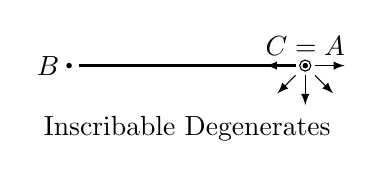
\begin{tikzpicture}
\node at (0,0) (A) {};
\node at (3,0) (B) {};
\draw[thick] (A) -- (B);
%\draw[->,-latex] (B)--({3+.5*cos(45)},{.5*sin(45)});
%\draw[->,-latex] (B)--({3+.5*cos(135)},{.5*sin(135)});
\draw[->,-latex] (B)--({3+.5*cos(180)},{.5*sin(180)});
\draw[->,-latex] (B)--({3+.5*cos(225)},{.5*sin(225)});
\draw[->,-latex] (B)--({3+.5*cos(270)},{.5*sin(270)});
\draw[->,-latex] (B)--({3+.5*cos(315)},{.5*sin(315)});
\draw[->,-latex] (B)--({3+.5*cos(0)},{.5*sin(0)});
%\draw[->,-latex] (B)--({3+.5*cos(90)},{.5*sin(90)});
\fill (0,0) circle (1pt);
\fill (3,0) circle (1pt);
\draw (3,0) circle (2pt);
\node[left] at (A) {$B$};
\node[above] at (B) {$C=A$};
\node at (1.5,-.8) {Inscribable Degenerates};
\end{tikzpicture}
\]
\noindent
(ii)
The exclusion from $\mf T_{\rm insc}$ of triangles
$((A,A,A);(\alpha,\beta,\gamma))$ with $(\alpha,\beta,\gamma)\neq(0,0,0)\pmod\pi$
is because they do
not appear as limits of families of nondegenerate inscribable classes.

\noindent
(iii) 
The definition of similarity in \eqref{(e)} agrees with the standard one
when all vertices are distinct, even when collinear. 
However it specifies distinct (degenerate) classes
where two or three vertices coincide, classified by their angle triples.
Though these classes may seem to appear out of thin air, 
we will see they are justified by our compactification
construction.
\end{Remarks}

\section{\Large The Torus}
In this section we construct a torus that naturally parameterizes inscribable triangle classes.
Let 
\[\R^3\lr\R^3/(\pi)^3\equiv\R/\pi\Z\times\R/\pi\Z\times\R/\pi\Z\] 
be the quotient, which is a smooth covering of abelian Lie groups by
\cite[Example 21.14]{Lee}.
In particular $\R^3/(\pi)^3$ is a smooth manifold, the $3$-torus.
Let
$\T\subset\R^3/(\pi)^3$ be the image %$(L+(\pi)^3)/(\pi)^3$ in $\R^3/(\pi)^3$ 
of the linear subspace $L:X+Y+Z=0$ of $\R^3$. Then $\T$ is a Lie subgroup by \cite[Theorem 21.27]{Lee}.
Noting that the sum of three numbers $\pmod\pi$ is uniquely defined $\pmod{3\pi}$,
we visualize $\T$ as the intersection with a solid cube of side-length $\pi$
of the four parallel planes $\frac k3(\pi,\pi,\pi)+L$ ($k=0,1,2,3$):
%$(k\pi,k\pi,-k\pi)+(-2k\pi/3,-2k\pi/3,4k\pi/3)+L=(k\pi,k\pi,-k\pi)+L$.
\begin{equation}\label{cube}
\tdplotsetmaincoords{60}{120}
\begin{tikzpicture}[scale=2,tdplot_main_coords]
% Draw the cube in the first octant
\draw (0,0,0) -- (1,0,0) -- (1,1,0) -- (0,1,0) -- cycle; % bottom face
\draw (0,0,0) -- (0,0,1) -- (0,1,1) -- (0,1,0) -- cycle; % left face
\draw (0,0,0) -- (1,0,0) -- (1,0,1) -- (0,0,1) -- cycle; % front face
\draw (1,1,0) -- (1,1,1) -- (0,1,1); % top edges
\draw (1,1,0) -- (1,0,0) -- (1,0,1); % right edges
\draw (0,0,1) -- (1,0,1) -- (1,1,1) -- (0,1,1) -- cycle; % top face
\draw[thick] (1,0,0) -- (0,1,0) -- (0,0,1) -- cycle;
\draw[thick] (1,1,0) -- (1,0,1) -- (0,1,1) -- cycle;
\draw[->,-latex] (0,0,0)--(2,0,0) node[left] {$X$};
\draw[->,-latex] (0,0,0)--(0,2,0) node[right] {$Y$};
\draw[->,-latex] (0,0,0)--(0,0,1.5) node[left] {$Z$};
\filldraw (0,0,0) circle (.5pt); 
\filldraw (1,1,1) circle (.5pt);
\filldraw (1,1,0) circle (.5pt);f
\filldraw (0,1,1) circle (.5pt);
\filldraw (1,0,1) circle (.5pt);
\filldraw (1,0,0) circle (.5pt) node[left] {$(\pi,0,0)$};
\filldraw (0,1,0) circle (.5pt) node[right] {$(0,\pi,0)$};
\filldraw (0,0,1) circle (.5pt) node[left] {$(0,0,\pi)$};
% Intersection with the plane X + Y + Z = 1
\fill[yellow, opacity=0.5] (1,0,0) -- (0,1,0) -- (0,0,1) -- cycle;
% Intersection with the plane X + Y + Z = 2
\fill[gray, opacity=0.5] (1,1,0) -- (1,0,1) -- (0,1,1) -- cycle;
\node at (1,1,-.5) {$\T\subset\R^3/(\pi)^3$};
\draw (.35,.85,1) arc (290:180:.5 and .1) node[right] {\footnotesize $X+Y+Z=-\pi\pmod{3\pi}$};
\draw (.2,.9,.2) arc (270:180:.5 and .1) node[right] {\footnotesize $X+Y+Z=\pi\pmod{3\pi}$};
\end{tikzpicture}
\end{equation}
The boundaries of the triangular regions, where one angle is
$0\pmod\pi$, are identified
on opposite faces of the cube, and all 8 vertices, where all
angles are $0\pmod\pi$, are identified to a single point.

\begin{Lemma}\label{torus}
The Lie subgroup $\T\subset\R^3/(\pi)^3$ is naturally isomorphic to a $2$-torus.
\end{Lemma}

\begin{proof}
The identifications of $\R^3/(\pi)^3$ shows the two triangles of $\T$ form a standard 
torus polygon:
\[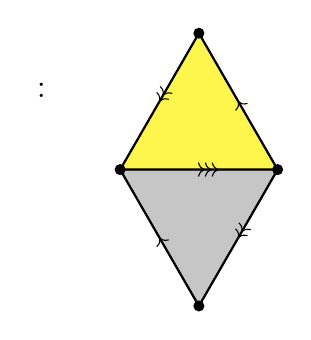
\begin{tikzpicture}[scale=2]
\coordinate (A) at (-1/2,0);
\coordinate (B) at (0,{sqrt(3)/2});
\coordinate (C) at (1/2,0);
\coordinate (D) at (0,{-sqrt(3)/2});
\draw[thick] (A)--(B)--(C)--(D)--(A)--(C);
\fill (A) circle (1pt);
\fill (B) circle (1pt);
\fill (C) circle (1pt);
\fill (D) circle (1pt);
\draw[->>] (B)--(-1/4,{sqrt(3)/4});
\draw[->>] (C)--(1/4,{-sqrt(3)/4});
\draw[->>>] (A)--(1/8,0);
\draw[->] (C)--(1/4,{sqrt(3)/4});
\draw[->] (D)--(-1/4,{-sqrt(3)/4});
\begin{scope}[on background layer]
\draw[fill=darkgray!30] (A)--(D)--(C)--(A);
\draw[fill=yellow!70] (A)--(B)--(C)--(A);
\end{scope}
\node at (-1,.5) {\large $\T:$};
\end{tikzpicture}\]
\end{proof}

Since we will show $\T$ is a moduli space in an algebrogeometric context, we record the following.
\begin{Corollary}\label{algvar}
$\T$ is an abelian linear algebraic group.
In particular it is an algebraic variety, and contains closed subgroups 
corresponding to linear subspaces
in \eqref{cube}.
\end{Corollary}

\begin{proof}
Since $\T$ is compact, the first statement is \cite[Ch.5, 2.5, Theorem 12]{OV}.
By the corollary to that theorem there is a one-to-one correspondence
between Lie subgroups and closed algebraic subgroups, and we
obtain the second statement since every linear subspace of 
$\R^3$ is a Lie subgroup.
\end{proof}

\section{\Large Triangle Classes on the Torus}

The following theorem shows $\T$ is a moduli space of inscribed triangle classes.

\begin{Theorem}\label{map}
The natural map 
\begin{align*}
\rho:[\mf T_{\rm insc}]&\lr\T\subset\R^3/(\pi)^3\\
[\left((A,B,C);(\alpha,\beta,\gamma)\right)]&\lm(\alpha,\beta,\gamma)\pmod\pi
\end{align*} 
is a bijection, taking positively oriented classes to the subset $X+Y+Z=\pi\pmod{3\pi}$ of $\R^3/(\pi)^3$,
negatively oriented classes to $X+Y+Z=-\pi\pmod{3\pi}$,
and degenerate classes to the boundary $\alpha\beta\gamma=0\pmod\pi$ in \eqref{cube}.
\end{Theorem}

\begin{proof}
The theorem says that a labeled, oriented, possibly-degenerate 
inscribable class is completely determined
by its triple of angles $\pmod\pi$; that every triple
$\pmod\pi$ arises from some class; and that the two shaded triangular regions in
\eqref{cube} correspond to the two possible orientations.

All three angles of a nondegenerate class belong to either $(0,\pi)$ or $(-\pi,0)$,
depending on orientation, so its image is in the interior $\alpha\beta\gamma\neq 0$ of $\T$,
and is uniquely determined by its angle values $\pmod\pi$ together with its orientation.
If the class is positively oriented then $\alpha+\beta+\gamma=\pi\pmod{3\pi}$,
so the image is in the yellow region in \eqref{cube},
and if negatively oriented $\alpha+\beta+\gamma=-\pi\pmod{3\pi}$, in the
gray region. 
Therefore $\rho$ distinguishes orientation, and is injective on nondegenerate classes.

A degenerate class with $\gamma=0$ has form $[(A,A,C);(\alpha,-\alpha,0)]$ with
$\alpha\in(-\pi,\pi]$, and maps to the identified faces of the cube \eqref{cube} parallel
to the $XY$-plane. By definition
$\rho([(A,A,C);(\alpha,-\alpha,0)])=\rho([(A',A',C');(\alpha',-\alpha',0)])$ if and only if 
$\alpha'=\alpha\pm\pi$, so we may assume $\alpha>0$ and $\alpha'=\alpha-\pi$.
Since there are only two, the vertices automatically differ by a nonzero complex constant, 
and since the interior angles are equal $\pmod\pi$, the triangles are similar
by Definition~\ref{triangles}\eqref{(e)}.
Clearly
this applies to the non-equiangular degenerates $\alpha=0$ and $\beta=0$ as well,
which go to the faces of the cube parallel to the $YZ$ and $XZ$-planes, respectively.
Thus $\rho$ remains injective if we include these classes.
The solitary equiangular degenerate class is $[(1,1,1);(0,0,0)]$ maps to $(0,0,0)\pmod\pi$,
and since this point has not been taken, we conclude $\rho$ is injective in general.

If $\alpha+\beta+\gamma=\pi\pmod{3\pi}$ and $\alpha\beta\gamma\neq 0\pmod\pi$ in $\T$
then there exist real representatives in $(0,\pi)$ adding to $\pi$, and these are
the angles of a positively oriented triangle, by Euclid. Similarly if the sum is $-\pi$
we find a negatively oriented triangle. Therefore 
$\rho$ is surjective on the interior regions of $\T$, dividing positively and negatively oriented
classes as above.
If $\gamma=0$ and $\alpha\neq 0\pmod\pi$ then $(\alpha,\beta,\gamma)\in\T$ is in the image of
the class $[(A,A,C);(\alpha,-\alpha,0)]$, and similarly if $\alpha=0$ or $\beta=0$.
We conclude $\rho$ is surjective, hence bijective, and divides classes as claimed.
\end{proof}

\begin{Remark}
Theorem~\ref{map} naturally identifies the set $[\mf T_{\rm insc}]$ with the variety $\T$, so it is
unsurprising that $\T$ is a fine moduli space of labeled, oriented, possibly-degenerate
inscribable classes, a result we prove below (Corollary~\ref{moduli}).
It follows that the interior $\alpha\beta\gamma\neq 0$ of $\T$ 
is a fine space for the nondegenerate classes, and $\T$ is its compactification.
%The latter result is well-known, see \cite[1.1.9 Exer. 1.30]{Beh}, but we justify it below.
%Thus $\T$ is a compactification of this fine moduli space.
\end{Remark}

\subsection{\bf Degenerates and Families}
The degenerate classes in $[\mf T_{\rm insc}]$ map to the boundary points $\alpha\beta\gamma=0\pmod\pi$
in $\T$. 
To see how they arise as inscribed triangles in families parameterized by $\T$ we 
will split the map $\rho$ with an explicit family of inscribed triangle classes over $\T$.
First, a lemma.


\begin{Lemma}\label{chord}
For points $B$ and $C$ on a circle, let $\Arc(BC)$ be the {\it oriented} (counterclockwise)
arc from $B$ to $C$ in radians.
Suppose $((A,B,C);(\alpha,\beta,\gamma))$ is nondegenerate and inscribed in a circle.
Then $\alpha=\frac 12\Arc(BC)\pmod\pi$, 
and $\alpha$ equals the oriented angle from the tangent line at $B$ to 
the chord $BC$, or alternatively from $BC$ to the tangent at $C$, measured on the side opposite $A$.
\end{Lemma}

\begin{proof}
The positively oriented case $\alpha=\frac 12\Arc(BC)$ is
Proposition 20 of Euclid's Book III, which states,
{\it In a circle the angle at the center is double the angle at 
the circumference when the angles have the same circumference as base} (\cite{Euclid}). 
%, see also \cite{DJ98}.
In the negatively oriented case $\alpha'<0$ we have $\alpha'=-\frac 12\Arc(CB)=\frac 12(\Arc(BC)-2\pi)=\frac 12(\Arc(BC)-\pi)$,
so $\alpha'=\frac 12\Arc(BC)\pmod\pi$, as desired. 

Diagram \eqref{alpha} shows how to compute the opposing angle from the tangent at $B$
to the chord $BC$ using similar triangles $MOB\sim MBI$. The last statement is immediate.
\begin{equation}
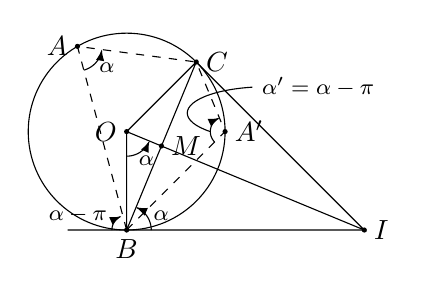
\begin{tikzpicture}[scale=1.25]\label{alpha}
\coordinate (O) at (0,0) node[left] at (O) {$O$};
\coordinate (B) at (0,-1) node[below] at (B) {$B$};
\coordinate (C) at ({1/sqrt(2)},{1/sqrt(2)}) node[right] at (C) {$C$};
\coordinate (M) at ({1/(2*sqrt(2))},{(-sqrt(2)+1)/(2*sqrt(2))}) node[right] at (M) {$M$};
\coordinate (I) at ({(2+sqrt(2))/sqrt(2)},-1) node[right] at (I) {$I$};
\coordinate (A) at (-1/2,{sqrt(3)/2}) node[left] at (A) {$A$};
\coordinate (A') at (1,0) node[right] at (A') {$A'$};
\draw (O) circle (1);
\draw (O)--(B)--(C)--(O)--(I)--(C);
\draw (I)--(-.6,-1);
\draw[dashed] (B)--(A)--(C);
\draw[dashed] (B)--(A')--(C);
\fill (O) circle (.75pt);
\fill (B) circle (.75pt);
\fill (C) circle (.75pt);
\fill (M) circle (.75pt);
\fill (I) circle (.75pt);
\fill (A) circle (.75pt);
\fill (A') circle (.75pt);
\draw[domain=0:1.178097,->,-latex] plot ({.25*cos(deg(\x))},{-1+.25*sin(deg(\x))}); %bottom right alpha
\draw[domain=-3.141593:-4.31969,->,-latex] plot ({.15*cos(deg(\x))},{-1+.15*sin(deg(\x))}); %bottom left
\draw[domain=-1.570796:-.392699,->,-latex] plot ({.25*cos(deg(\x))},{.25*sin(deg(\x))});
\draw[domain=-1.308997:-.1309,->,-latex] plot ({-1/2+.25*cos(deg(\x))},{(sqrt(3)/2)+.25*sin(deg(\x))});
\draw[domain=-135:-247.5,->,-latex] plot ({1+.15*cos(\x)},{.15*sin(\x)}); %right alpha'
\draw (.85,0) arc (-135:-260:.8 and .8/3) node[right] {\footnotesize $\alpha'=\alpha-\pi$}; %For alpha' arc.
\node at (.2,-.3) {\footnotesize $\alpha$};
\node at (.35,-.85) {\footnotesize $\alpha$};
\node at (-.2,.65) {\footnotesize $\alpha$};
\node[left] at (-.1,-.85) {\footnotesize $\alpha-\pi$};
\end{tikzpicture}
\end{equation}
\end{proof}


The next result gives an inscribed family over $\T$.

\begin{Theorem}\label{family}
The map $\rho$ of Theorem~\ref{map} has inverse
\begin{align*}
\sigma:\T&\lr[\mf T_{\rm insc}]\\
(\alpha,\beta,\gamma)\pmod\pi&\lm\left[(e^{2\beta\i},e^{-2\alpha\i},1);(\alpha,\beta,\gamma)\right]
\end{align*}
where the interior angles on the right are real representatives in $(-\pi,\pi]$ 
adding to $\pm\pi$, of the same sign when $\alpha\beta\gamma\neq 0$.
\end{Theorem}

\begin{proof}
The choice of real representatives when $\alpha\beta\gamma\neq 0$ is 
unique by diagram \eqref{cube}.
The map $\sigma$ as stated clearly splits $\rho$ if it is well-defined, i.e.,
if its stated images are actually classes as defined in Definition~\ref{triangles}.
We illustrate $\sigma$ on nondegenerate triples, with the oriented arcs computed using 
the vertices' arguments:
\begin{equation}\label{euclid}
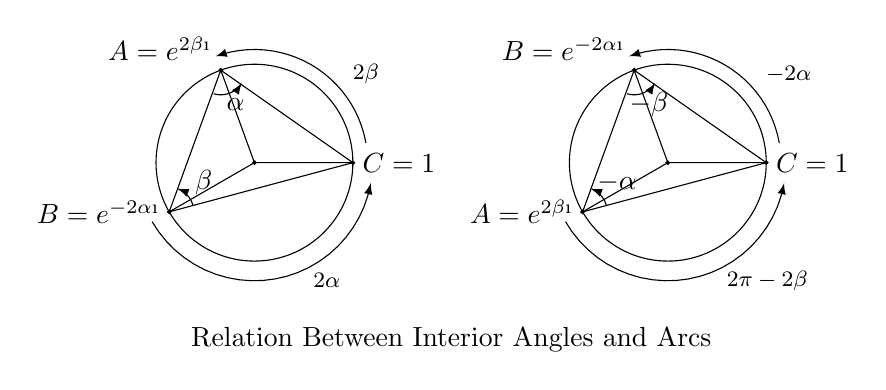
\begin{tikzpicture}[scale=1.25]
\coordinate (A) at ({cos(110)},{sin(110)});
\coordinate (B) at ({cos(210)},{sin(210)});
\coordinate (C) at (1,0);
\draw (0,0) circle (1);
\filldraw (1,0) circle (.5pt);
\filldraw (A) circle (.5pt);
\filldraw (B) circle (.5pt);
\filldraw (0,0) circle (.5pt);
\draw (A)--(B)--(C)--(A);
\draw (1,0)--(0,0)--(A);
\draw (0,0)--(B);
\draw[domain=10:110,->,-latex] plot ({1.15*cos(\x)},{1.15*sin(\x)}); %arc CA
\draw[domain=253:328,->,-latex] plot ({cos(110)+.25*cos(\x)},{sin(110)+.25*sin(\x)}); %angle alpha
\draw[domain=15:70,->,-latex] plot ({cos(210)+.25*cos(\x)},{sin(210)+.25*sin(\x)}); %angle beta
\draw[domain=-150:-10,->,-latex] plot ({1.2*cos(\x)},{1.2*sin(\x)}); %arc BC
\node[right] at (.9,.9) {\footnotesize $2\beta$};
\node[right] at (.5,-1.2) {\footnotesize $2\alpha$};
\node at ({cos(210)+.35},{sin(210)+.3}) {$\beta$};
\node at ({cos(110)+.15},{sin(110)-.35}) {$\alpha$};
\node[right] at (C) {$C=1$};
\node[left] at (B) {$B=e^{-2\alpha\i}$};
\node[above left] at (A) {$A=e^{2\beta\i}$}; %%%%%%%%%%%%%%%Break for second picture, shifted 4.2
\coordinate (D) at ({4.2+cos(110)},{sin(110)});
\coordinate (E) at ({4.2+cos(210)},{sin(210)});
\coordinate (F) at (5.2,0);
\draw (4.2,0) circle (1);
\filldraw (5.2,0) circle (.5pt);
\filldraw (D) circle (.5pt);
\filldraw (E) circle (.5pt);
\filldraw (4.2,0) circle (.5pt);
\draw (D)--(E)--(F)--(D);
\draw (5.2,0)--(4.2,0)--(D);
\draw (4.2,0)--(E);
\draw[domain=10:110,->,-latex] plot ({4.2+1.15*cos(\x)},{1.15*sin(\x)}); %arc CB
\draw[domain=253:328,->,-latex] plot ({4.2+cos(110)+.25*cos(\x)},{sin(110)+.25*sin(\x)}); %angle alpha<0
\draw[domain=15:70,->,-latex] plot ({4.2+cos(210)+.25*cos(\x)},{sin(210)+.25*sin(\x)}); %angle beta<0
\draw[domain=-150:-10,->,-latex] plot ({4.2+1.2*cos(\x)},{1.2*sin(\x)}); %arc AC
\node[right] at (5.1,.9) {\footnotesize $-2\alpha$};
\node[right] at (4.7,-1.2) {\footnotesize $2\pi-2\beta$};
\node at ({4.2+cos(210)+.35},{sin(210)+.3}) {$-\alpha$};
\node at ({4.2+cos(110)+.15},{sin(110)-.35}) {$-\beta$};
\node[right] at (F) {$C=1$};
\node[left] at (E) {$A=e^{2\beta\i}$};
\node[above left] at (D) {$B=e^{-2\alpha\i}$};
\node at (2,-1.8) {Relation Between Interior Angles and Arcs};
\end{tikzpicture}
\end{equation}
The interior angles in \eqref{euclid} are correct by Lemma~\ref{chord}. %In particular, on the right $\alpha,\beta<0$.
This calculation can be used in lieu of conditions (ii)-(iv) of Definition~\ref{triangles}\eqref{(a)},
which simply ensure that given vertices and interior angles are compatible.
Therefore $\sigma$ is well-defined on $\alpha\beta\gamma\neq 0$.
If $(\alpha,\beta,0)\in\T$ and $\alpha\neq 0\pmod\pi$, then $\beta=-\alpha$, so
\[\sigma(\alpha,\beta,\gamma)=[(e^{-2\alpha\i},e^{-2\alpha\i},1);(\alpha,-\alpha,0)]\] which is well-defined.
Similarly if $\alpha=0$ and $\beta\neq 0$, or $\beta=0$ and $\alpha\neq 0$, we find the image
of $\sigma$ is $[(e^{2\beta\i},1,1);(0,\beta,-\beta)]$ and $[(1,e^{-2\alpha\i},1);(\alpha,0,-\alpha)]$,
respectively, both well-defined. Finally the remaining point $(0,0,0)\in\T$ maps to $[(1,1,1);(0,0,0)]$,
as desired. This completes the proof.
\end{proof}

\begin{Remark}
The map $\sigma$ gives inscribed triangles over $\T$
naturally representing every class in $[\mf T_{\rm insc}]$.
The existence of such a family is an important feature of a (fine) moduli space,
a sort of testimonial to the fine-ness.
But since we have {\it identified} $\T$ with the classes $[\mf T_{\rm insc}]$ via $\rho$, $\T$ itself
provides such a family, tautologically. 
Theorem~\ref{family} goes further by specifying an explicit set of triangle representatives. 
We define families more rigorously in Section~\ref{moduliquotient}.
\end{Remark}

\begin{Example}\label{arise}
We show how the degenerate classes arise in inscribed families defined by a fixed chord.
Fix $\alpha_0\in(0,\pi)$, then
$\sigma$ sends the ``circle'' of points $(\alpha_0,\beta,\gamma)\pmod\pi\in\T$ 
to the family
\[\{[(e^{2\beta\i},e^{-2\alpha_0\i},1);(\alpha_0,\beta,\gamma)]:\beta\in[0,\pi-\alpha_0]\cup[-\alpha_0,0]\}
\subset[\mf T_{\rm insc}]\]
The chord $BC$ is fixed,
and various $\beta$ locate $A$ anywhere on the circle. In particular
$\beta=0$ and $\beta=-\alpha_0\pmod\pi$ field the degenerates
$[(1,e^{-2\alpha_0\i},1);(\alpha_0,0,-\alpha_0)]$  and $[(e^{-2\alpha_0\i},e^{-2\alpha_0\i},1);(\alpha_0,-\alpha_0,0)]$,
respectively; both $BC$ but with a different doubled vertex.
The family consists of inscribed triangles on the unit circle
with fixed chord $BC$, including the degenerate triangles, the chord $BC$ itself.
In this way each degenerate inscribable class -- when inscribed --
corresponds to a specific chord 
with a double point at one end or the other.

By the second part of Lemma~\ref{chord} the degenerate inscribed class
$[(A,B,A);(\alpha,0,-\alpha)]$ above can be drawn as
\begin{equation}\label{deginsc}
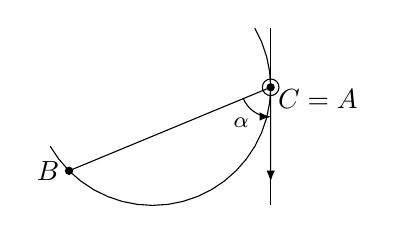
\begin{tikzpicture}[scale=1.5]
\coordinate (B) at ({-sqrt(2)/2},{-sqrt(2)/2}) node[left] at (B) {$B$};
\coordinate (C) at (1,0);
\node at (1.4,-.1) {$C=A$};
\fill (B) circle (1pt);
\fill (C) circle (1pt);
\draw (C) circle (2pt);
\draw (B)--(C);
\draw[->,-latex] (C)--(1,-.8);
\draw (1,-1)--(1,.5);
\draw[domain=-150:30] plot ({cos(\x)},{sin(\x)});
\draw[domain=-2.748894:-1.570796,->,-latex] plot ({1+.25*cos(deg(\x))},{.25*sin(deg(\x))});
\node at (.75,-.3) {\footnotesize $\alpha$};
%\node at (0,-1.5) {The degenerate inscribed class $((A,B,A);(\alpha_0,0,-\alpha_0))$};
\end{tikzpicture}
\end{equation}
Different degenerate inscribable classes
can be distinguished geometrically using directions from the double point,
as pictured earlier:
\begin{equation}\label{pixie}
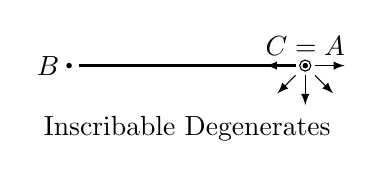
\begin{tikzpicture}
\node at (0,0) (A) {};
\node at (3,0) (B) {};
\draw[thick] (A) -- (B);
%\draw[->,-latex] (B)--({3+.5*cos(45)},{.5*sin(45)});
%\draw[->,-latex] (B)--({3+.5*cos(135)},{.5*sin(135)});
\draw[->,-latex] (B)--({3+.5*cos(180)},{.5*sin(180)});
\draw[->,-latex] (B)--({3+.5*cos(225)},{.5*sin(225)});
\draw[->,-latex] (B)--({3+.5*cos(270)},{.5*sin(270)});
\draw[->,-latex] (B)--({3+.5*cos(315)},{.5*sin(315)});
\draw[->,-latex] (B)--({3+.5*cos(0)},{.5*sin(0)});
%\draw[->,-latex] (B)--({3+.5*cos(90)},{.5*sin(90)});
\fill (0,0) circle (1pt);
\fill (3,0) circle (1pt);
\draw (3,0) circle (2pt);
\node[left] at (A) {$B$};
\node[above] at (B) {$C=A$};
\node at (1.5,-.8) {Inscribable Degenerates};
\end{tikzpicture}
\end{equation}
Here $\alpha\in[0,\pi)$ is the angle between $BC$ and an arrow on the right.
This is the complete range of possibilities since e.g. $[(A,B,A);(\alpha,0,-\alpha)]=[(A,B,A);(-\alpha,0,\alpha)]$.
\end{Example}

The point $(0,0,0)\in\T$, which is a limit obtained by collapsing a double point's solitary vertex,
uniquely corresponds to the degenerate equiangular class $[(1,1,1);(0,0,0)]$.
Thus we distinguish three degenerate class types:
\begin{equation}
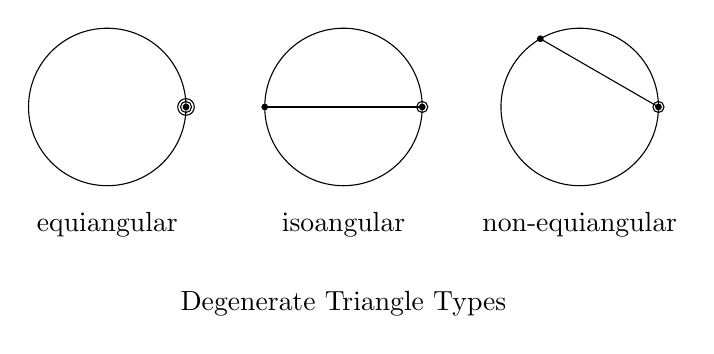
\begin{tikzpicture}\label{degenerates} 
\filldraw (-2,0) circle (1pt);
\draw (-2,0) circle (2pt);
\draw (-2,0) circle (3pt);
\filldraw (1,0) circle (1pt);
\draw (1,0) circle (2pt);
\filldraw (-1,0) circle (1pt);
\filldraw (4,0) circle (1pt);
\draw (4,0) circle (2pt);
\filldraw (2.5,{sqrt(3)/2}) circle (1pt);
\draw (-3,0) circle (1cm);
\draw (0,0) circle (1cm);
\draw (3,0) circle (1cm);
\draw (-1,0)--(1,0);
\draw (4,0)--(2.5,{sqrt(3)/2});
\node at (-3,-1.5) {equiangular};
\node at (0,-1.5) {isoangular};
\node at (3,-1.5) {non-equiangular};
\node at (0,-2.5) {Degenerate Triangle Types};
\end{tikzpicture}
\end{equation}


As mentioned in the introduction,
this way of defining similarity for degenerate classes in a compactification of 
triples of points in the plane appears in a much more general and far-reaching context
in the work of \cite{Ful94}, \cite{AxSi94}, and \cite{Sinha} on configuration spaces, especially
of finitely many points on manifolds.

\subsubsection{\bf The Missing Degenerates}\label{missing}
The equiangular point $(0,0,0)\pmod\pi\in\T$ conceals
the entire set of nontrivial (degenerate) collinear {\it un}inscribable classes, whose angles are all $0\pmod\pi$, and 
which are classified by the ratios of their side lengths $|\a|,|\b|,|\c|$.
These are used in \cite[1.1.10]{Beh} to construct
a different compactification
of labeled, oriented, nondegenerate classes, called a {\it bipyramid}. The construction is similar to ours,
describing two triangular regions and gluing them along the degenerate (collinear) boundaries.
The resulting space is a topological sphere, 
the bipyramid (\cite[Figure 1.21]{Beh}), later recast as the Riemann sphere.

Since neither the torus nor the sphere incorporates all notions of
degenerate configurations of three vertices, neither gives a ``final'' compactification of 
the space of labeled, oriented, nondegenerate triangle classes.
And there are more:
We have also omitted non-equiangular ``triple points'' of the form $[(1,1,1);(\alpha,\beta,\gamma)]$,
which are realized as limits of the 
nondegenerate triangles in a fixed class as the side vectors are scaled to zero while the angles are held
constant.
Both sets are excluded from our construction
because they do not arise in (limits of) inscribed triangle families.

In \cite{BGGL} we show that a unification exists, called {\it Dyck's surface}, which is
the blowup of the sphere at three points 
(``pinched points'' in \cite{Beh}), or the torus at a single point (the degenerate equiangular point).

\section{\Large Group-Theoretic Interpretation of Triangle Types}\label{disting}

In this section we show
the group structure of $\T$, given by addition of angle triples $\pmod\pi$, 
is compatible with triangle types, in the sense that the latter form
basic algebraic structures: elements of finite order, subgroups, and cosets.
The identity of $\T$ is the class $(0,0,0)$ of the degenerate equiangular class $[(1,1,1);(0,0,0)]$.
The diagram below illustrates the main triangle types.
\begin{equation}\label{diamond}
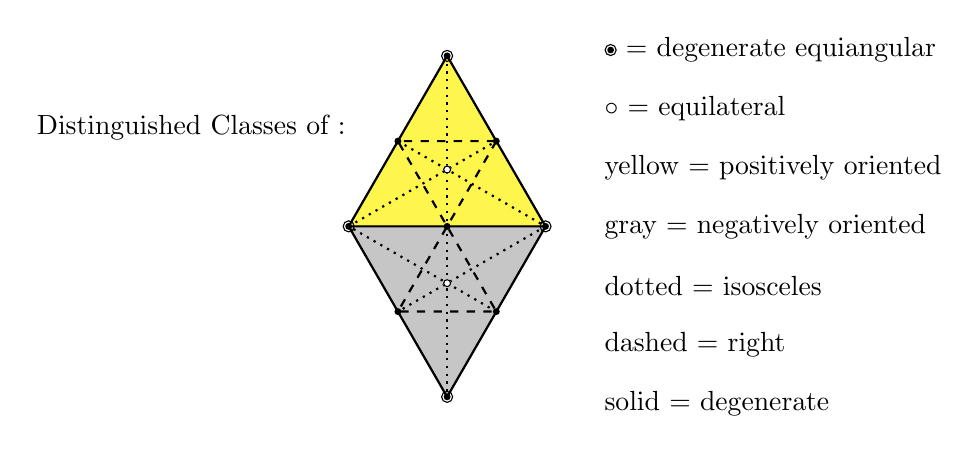
\begin{tikzpicture}[scale=2.5]
\coordinate (A) at (-1/2,0); %left
\coordinate (B) at (0,{sqrt(3)/2}); %top
\coordinate (C) at (1/2,0); %right
\coordinate (D) at (0,{-sqrt(3)/2}); %bottom
\coordinate (AB) at (-1/4,{sqrt(3)/4}); 
\coordinate (BC) at (1/4,{sqrt(3)/4});
\coordinate (AC) at (0,0);
\coordinate (AD) at (-1/4,{-sqrt(3)/4});
\coordinate (CD) at (1/4,{-sqrt(3)/4});
\draw[thick] (A)--(B)--(C)--(D)--(A)--(C);
\fill (A) circle (.5pt);
\fill (B) circle (.5pt);
\fill (C) circle (.5pt);
\fill (D) circle (.5pt);
\fill (AC) circle (.5pt);
\fill (AB) circle (.5pt);
\fill (BC) circle (.5pt);
\fill (AD) circle (.5pt);
\fill (CD) circle (.5pt);
\draw[thick,dashed] (BC)--(AD)--(CD)--(AB)--(BC);
\draw[thick,dotted] (B)--(D);
\draw[thick,dotted] (CD)--(A)--(BC);
\draw[thick,dotted] (AB)--(C)--(AD);
\begin{scope}[on background layer]
\draw[fill=darkgray!30] (A)--(D)--(C)--(A);
\draw[fill=yellow!70] (A)--(B)--(C)--(A);
\end{scope}
\filldraw[white] (0,{sqrt(3)/6}) circle (.5pt);
\filldraw[white] (0,{-sqrt(3)/6}) circle (.5pt);
\draw (0,{sqrt(3)/6}) circle (.5pt);
\draw (0,{-sqrt(3)/6}) circle (.5pt);
\draw (A) circle (.8pt);
\draw (B) circle (.8pt);
\draw (C) circle (.8pt);
\draw (D) circle (.8pt);
\node[right] at (.75,.9) {$\tikz{\draw(0,0) circle (2pt);\filldraw (0,0) circle (1pt);}$ $=$ degenerate equiangular};
\node[right] at (.75,.6) {$\circ$ $=$ equilateral};
\node[right] at (.75,.3) {yellow $=$ positively oriented};
\node[right] at (.75,0) {gray $=$ negatively oriented};
\node[right] at (.75,-.3) {dotted $=$ isosceles};
\node[right] at (.75,-.6) {dashed $=$ right};
\node[right] at (.75,-.9) {solid $=$ degenerate};
\node at (-1.3,.5) { Distinguished Classes of $\T$:};
\end{tikzpicture}
\end{equation}

Let ${\sf  I}_X$, ${\sf  D}_X$, ${\sf R}_X$ for $X=A,B,C$ denote the points of $\T$
corresponding to 
isosceles, degenerate, and right triangles, with distinguished vertex $X$.
The standard triangle classes have the following algebraic interpretations,
for $X=A,B,C$. 
\begin{enumerate}[\rm(a)]
\item
Each ${\sf I}_X\leq\mbb T$ is a subgroup isomorphic to $\R/(\pi)$.
They are:
\[{\sf I}_A=\{(-2\beta,\beta,\beta)\},\,{\sf I}_B=\{(\alpha,-2\alpha,\alpha)\},\,
{\sf I}_C=\{(\alpha,\alpha,-2\alpha)\}\]
\item
Each ${\sf D}_X\leq\mbb T$ is a subgroup isomorphic to $\R/(\pi)$.
They are:
\[{\sf D}_A=\{(0,\beta,-\beta)\},\,
{\sf D}_B=\{(\alpha,0,-\alpha)\},\, {\sf D}_C=\{(\alpha,-\alpha,0)\}\]
\item
Each ${\sf R}_X\subset\mbb T$ is a coset of ${\sf D}_X$, consisting of the
elements of order two $\pmod{D_X}$:
\begin{align*}
{\sf R}_A&=(\tfrac\pi 2,\tfrac\pi 4,\tfrac\pi 4)+{\sf D}_A=\{(\tfrac\pi 2,\tfrac\pi 4+\beta,\tfrac\pi 4-\beta)\}\\
{\sf R}_B&=(\tfrac\pi 4,\tfrac\pi 2,\tfrac\pi 4)+{\sf D}_B=\{(\tfrac\pi 4+\alpha,\tfrac\pi 2,\tfrac\pi 4-\alpha)\}\\
{\sf R}_C&=(\tfrac\pi 4,\tfrac\pi 4,\tfrac\pi 2)+{\sf D}_C=\{(\tfrac\pi 4+\alpha,\tfrac\pi 4-\alpha,\tfrac\pi 2)\}
\end{align*}
\item
The positive and negative equilateral classes are inverses, each of order $3$: 
$\pm(\tfrac\pi 3,\tfrac\pi 3,\tfrac\pi 3)$ in 
the intersection ${\sf I}_A\cap{\sf I}_B\cap{\sf I}_C$.
\item
The three degenerate non-equiangular isosceles classes are of order $2$, given by
\[\{(0,\tfrac\pi 2,\tfrac\pi 2),(\tfrac\pi 2,0,\tfrac\pi 2),(\tfrac\pi 2,\tfrac\pi 2,0)\}\]
Each is the unique order-two element of the subgroups ${\sf D}_A,{\sf D}_B,{\sf D}_C$,
respectively.
\item
The six nondegenerate right-isosceles classes
\[\left\{\pm(\tfrac\pi 2,\tfrac\pi 4,\tfrac\pi 4),\pm(\tfrac\pi 4,\tfrac\pi 2,\tfrac\pi 4),
\pm(\tfrac\pi 4,\tfrac\pi 4,\tfrac\pi 2)\right\}\]
are generators of three cyclic groups of order $4$.
Each group contains one of the three degenerate non-equiangular isosceles class (of order $2$).
\end{enumerate}

\section{\Large Ratios}
The natural metric on 
our model computes ratios of different triangle types,
easily read off of \eqref{diamond} after multiplicities are encoded (as necessary).
If we normalize the side-length of the yellow equilateral triangle at $2$, we
find the isosceles classes measure $2\times (6\times\sqrt 3)=12\sqrt 3$,
the right classes $1\times (3\times 2)=6$, and
the acute-isosceles and obtuse-isosceles both $2\times(6\times \sqrt 3/2)=6\sqrt 3$.
Since the acute classes are inside the dashed triangles, 
%and the generic elements of each have the same multiplicity, 
the obtuse to acute ratio is $(3:1)$.
The
isosceles to right ratio is $(2\sqrt 3:1)$, and the
obtuse-isosceles to acute-isosceles ratio is $(1:1)$.
We do not think this model is any more ``metrically correct'' than other models, such
as the sphere in \cite{Beh} and \cite{ES15}. In fact, we believe there are strong arguments that both are incorrect,
essentially because both omit important degenerate classes,
as mentioned in Subsubsection~\ref{missing}.

\section{\Large Group Action}\label{groupoid}

A nondegenerate scalene triangle has a single absolute similarity class,
but twelve labeled, oriented similarity classes:
six corresponding to the ways of
assigning the three angles assigned to the three vertices,
and two for each orientation.
In general $\T$ admits a group action by $D_6=\br{r,s}$ whose orbits are classes that
are {\it absolutely similar}, i.e., similar as unoriented, unlabeled 
inscribable classes.
This is depicted in diagram \eqref{hex}:

\begin{equation}\label{hex}
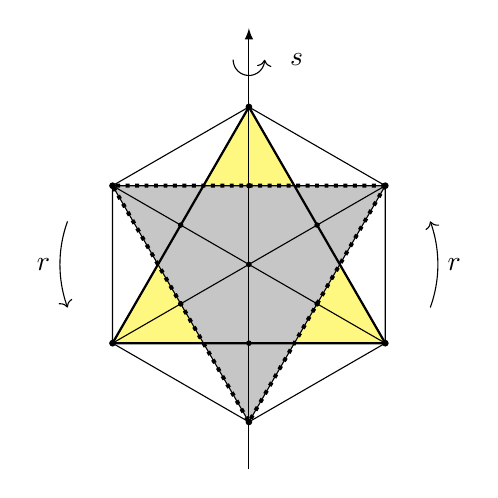
\begin{tikzpicture}[scale=2]%Hexagon 
\coordinate (O) at (0,0); \fill (O) circle (.5pt);
\coordinate (A) at ({cos(30)},{sin(30)}); \filldraw (A) circle (.5pt);
\coordinate (B) at ({cos(90)},{sin(90)}); \filldraw (B) circle (.5pt);
\coordinate (C) at ({cos(150)},{sin(150)}); \filldraw (C) circle (.5pt);
\coordinate (D) at ({cos(210)},{sin(210)}); \filldraw (D) circle (.5pt);
\coordinate (E) at ({cos(270)},{sin(270)}); \filldraw (E) circle (.5pt);
\coordinate (F) at ({cos(330)},{sin(330)}); \filldraw (F) circle (.5pt);
\coordinate (AC) at ({(1/2)*cos(30)},{(1/2)*sin(30)}); \fill (AC) circle (.5pt);
\coordinate (CE) at ({(1/2)*cos(90)},{(1/2)*sin(90)}); \fill (CE) circle (.5pt);
\coordinate (EA) at ({(1/2)*cos(150)},{(1/2)*sin(150)}); \fill (EA) circle (.5pt);
\coordinate (BD) at ({(1/2)*cos(210)},{(1/2)*sin(210)}); \fill (BD) circle (.5pt);
\coordinate (DF) at ({(1/2)*cos(270)},{(1/2)*sin(270)}); \fill (DF) circle (.5pt);
\coordinate (FB) at ({(1/2)*cos(330)},{(1/2)*sin(330)}); \fill (FB) circle (.5pt);
\draw[thick] (B)--(D)--(F)--(B); %gold
\draw[line width=0.5mm, dotted] (A)--(C)--(E)--(A); %shadow
\draw[thin] (A)--(B)--(C)--(D)--(E)--(F)--(A); %hexagon
\draw[thin] (A)--(D);
\draw[thin] (B)--(E);
\draw[thin] (C)--(F);
\draw[thin,->,-latex] (0,-1.3)--(0,1.5); %axis
%arcs
\draw[domain=-180:0, ->] plot ({.1*cos(\x)},{1.3+.1*sin(\x)});
\draw[domain=-20:20, ->] plot ({.4+.8*cos(\x)},{.8*sin(\x)});
\draw[domain=160:200, ->] plot ({-.4+.8*cos(\x)},{.8*sin(\x)});
\node[right] at (.2,1.3) {$s$};
\node[right] at (1.2,0) {$r$};
\node[left] at (-1.2,0) {$r$};
%nodes
%shading
\begin{scope}[on background layer]
\draw[fill=yellow!50] (B)--(D)--(F)--(B);
\draw[fill=darkgray!30] (A)--(C)--(E)--(A);
\end{scope}
\end{tikzpicture}
\end{equation}
The explicit action on a general point is given by $r(\alpha,\beta,\gamma)=(-\beta,-\gamma,-\alpha)$
and $s(\alpha,\beta,\gamma)=(\beta,\alpha,\gamma)$.
The resulting transformation groupoid is $\T\times D_6$.
This result is \cite[Exercise 1.38]{Beh} for the bipyramid; the computation here is almost the same.
The quotient $\T/D_6$ is the (coarse) moduli set of absolute possibly-degenerate inscribable classes,
drawn in \eqref{stacky} with ``stacky'' multiplicities, which are the orders of the stabilizer subgroups.
\begin{equation}\label{stacky}
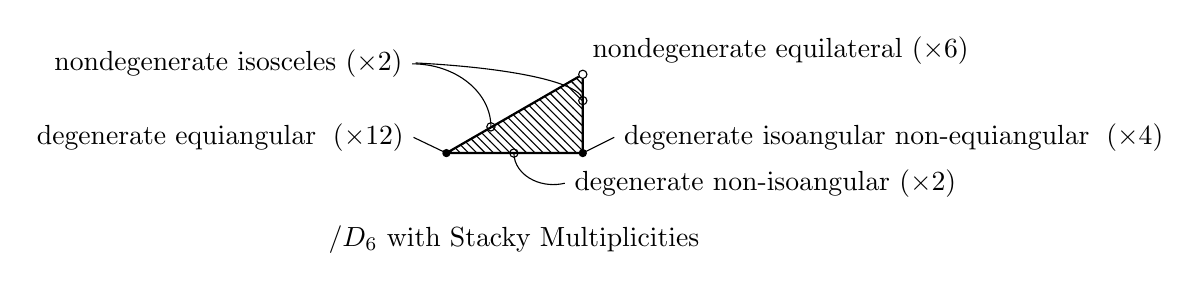
\begin{tikzpicture}
\coordinate (A) at (0,0);
\coordinate (B) at (0,1);
\coordinate (C) at ({-sqrt(3)},0);
\coordinate (D) at ({-sqrt(3)/3},2/3);
\draw[thick] (A)--(B)--(C)--(A);
\filldraw[white] (B) circle (1.5pt);
\fill (A) circle (1.5pt);
\draw (B) circle (1.5pt) node[above right] {nondegenerate equilateral $(\times 6)$};
\fill (C) circle (1.5pt);
%\fill (D) circle (1.5pt);
\draw (-14/12,1/3) arc (0:90:1 and .8) node[left] {nondegenerate isosceles $(\times 2)$};
\draw (0,2/3) arc (0:73:3 and .5); %to isosceles
\draw (-14/12,1/3) circle (1.5pt);
\draw (0,2/3) circle (1.5pt);
\draw (-7/8,0) circle (1.5pt);
\draw (-7/8,0) arc (180:73:.5 and -.4) node[right] {degenerate non-isoangular $(\times 2)$};
\draw (A)--(.4,.2) node[right] {degenerate isoangular non-equiangular\; $(\times 4)$}; 
\draw (C)--(-1.75-.4,.2) node[left] {degenerate equiangular\; $(\times 12)$};
\begin{scope}[on background layer]
%\draw[fill=darkgray!30] (A)--(B)--(C)--(A);
\draw[pattern=north west lines] (A)--(B)--(C)--(A);
\end{scope}
\node at (-7/8,-1.1) { $\T/D_6$ with Stacky Multiplicities};
\end{tikzpicture}
\end{equation}

\section{\Large Moduli Space and Quotient Stack}\label{moduliquotient}

We will now view $\T$ as a variety as per Corollary~\ref{algvar},
and prove it is a moduli space of labeled, oriented, possibly-degenerate inscribed classes
in the algebrogeometric setting.
We use the term {\it $\R$-variety} to mean a nonsingular, integral, separated scheme of finite type over $\R$.
Every $\R$-variety is a smooth manifold over $\R$. We write $\Var{\R}$ for the category of
$\R$-varieties, and in the following assume some elementary background in algebraic geometry
and category theory.

\begin{Definition}\label{families}\rm
If $B$ is an $\R$-variety, let $\pi_\T$ and $\pi_B$ be the projections on $\T\times_\R B$.
\begin{enumerate}[\rm (a)]
\item\label{a}
A {\it family in $\T$ over $B$} is a subvariety $F\subset \T\times_\R B$ such that
$\pi_B|_F:F\to B$ is an isomorphism.
\item\label{b}
The {\it pullback} $\phi^*(F/B)$ along a morphism $\phi:C\to B$
is the family $F_C:=(F\times_B C)/C$.
\item
The (contravariant) \textit{moduli functor of labeled, oriented, possibly-degenerate inscribable classes}
\[\FF_{\,\T}:\Var{\R}\to\Set\qquad\]
assigns to each $B\in\Var{\R}$ the set of families $F/B$ in $\T$, and
to each map $\phi:C\to B$ in $\Var{\R}$ the pullback of \eqref{b}.
\end{enumerate}
\end{Definition}

\begin{Remark}
Alternatively, a family is given by a morphism $f=(\alpha,\beta,\gamma):B\lr \R^3/(\pi)^3$ in $\Var{\R}$
whose image lies on $\T$.
That is, we assign to each $b\in B$ an
ordered triple $f(b)=(\alpha(b),\beta(b),\gamma(b))$, where $\alpha,\beta,\gamma:B\to\R/(\pi)$
are (regular) morphisms.
This phrasing
emphasizes the requirement that families vary continuously (regularly) over the points of $B$,
and is more in line with the definitions of families given in \cite{Beh} and other sources.
But it's the same:
Since $\T/\R$ is separated, the graph $F=\Gamma_f$ is closed in $B\times_\R\T$, and
since $f$ is regular, $\pi_B|_F:F\to B$ is an isomorphism.
Conversely \eqref{a} above is easily shown to define such a morphism $(\alpha,\beta,\gamma)$.
\end{Remark}

The following theorem, which shows $\T$ is a fine moduli space,
is at this point almost a formality. 

\begin{Theorem}\label{Theta}
The functor $\FF_{\,\T}$ is isomorphic to $\Hom_{\Var{\R}}(-,\T)$.
\end{Theorem}

\begin{proof}
We construct a natural transformation $\Theta:\FF_{\,\T}\to\Hom_{\Var{\R}}(-,\T)$.
A family $F/B$ defines a morphism $f:B\to\T$ by composing $(\pi_B|_F)^{-1}:B\to F$ 
with $\pi_\T:\T\times B\to\T$. This is a morphism since $\pi_B|_F$ is an isomorphism.
Define the component of $\Theta$ on the (arbitrary) base $B$ by $\Theta_B(F)=f$.
To prove $\Theta$ is a natural transformation we must show that a morphism
$\phi:C\to B$ determines a commutative diagram
\[\begin{tikzcd}[ampersand replacement=\&]
{\FF_{\,\T}(B)} \&\& {\Hom_{\Var{\R}}(B,\T)} \\
\\
{\FF_{\,\T}(C)} \&\& {\Hom_{\Var{\R}}(C,\T)}
\arrow["{\Theta_B}", from=1-1, to=1-3]
\arrow["\FF_{\,\T} (\phi)"', from=1-1, to=3-1]
\arrow["{\Hom_{\Var{\R}}(\phi,\T)}", from=1-3, to=3-3]
\arrow["{\Theta_C}"', from=3-1, to=3-3]
\end{tikzcd}\]
Suppose $F\in\FF_{\,\T}(B)$ defines the $B$-point $f:B\to\T$, as above.
Then $\Theta_B(F)=f$, and by definition $(\Hom_{\Var{\R}}(\phi,\T)\circ\Theta_B)(F)=f\circ\phi$.
On the other hand,
by definition $\FF_{\,\T}(\phi)(F)=F\times_B C=F_C$,
and $\Theta_C(F_C)$ is the composition $\pi_\T\circ(\pi_C|_{F_C})^{-1}$.
Suppose $(\eta,c)$ is a point of $F_C$, so that by definition of fiber product
$\pi_B(\eta)=\phi(c)$, and by definition of $f$, $f(\phi(c))=\pi_\T(\eta)$,
and $\pi_\T(\eta)=\pi_\T(\eta,c)$ by the associativity of the fiber product.
%We have $(\T\times_\R B)\times_B C=\T\times_\R(B\times_B C)=\T\times_\R C$,
%so if $\eta=(f(b),b)\in F$, 
Therefore $\Theta_C(F_C)(c)\df\pi_\T\circ(\pi_C|_{F_C})^{-1}(c)=\pi_\T(\eta,c)=f(\phi(c))$.
We conclude $\Theta_C\circ\FF_{\,\T}(\phi)=f\circ\phi$, and since $F/B$ was arbitrary,
this shows the diagram commutes, hence
$\Theta$ is a natural transformation.

We invert $\Theta$ by taking $f\in\Hom_{\Var{\R}}(B,\T)$ to
the family $F/B\in\FF_{\,\T}(B)$ defined by the graph of $f$, which is a subvariety of $\T\times_\R B$
since $\R$-varieties are separated. 
The proof that this inverts $\Theta$ is straightforward, and 
shows $\FF_{\,\T}$ and $\Hom_{\Var{\R}}(-,\T)$ are isomorphic.
\end{proof}

\begin{Corollary}\label{moduli}
$\T$ is a fine moduli space for the set of all labeled, oriented,
possibly-degenerate inscribable triangle classes,
which is a compactification of $\T^\circ=\T-\{\alpha\beta\gamma=0\}$, which in turn
is the fine moduli space of labeled, oriented, nondegenerate inscribable classes.
In particular, the family $[\mf T_{\rm insc}]=\T$ is a universal family, given explicitly by $\sigma$
in Theorem~\ref{map}.
\end{Corollary}

\begin{proof}
Already there is a bijection between labeled, oriented, possibly-degenerate inscribable classes
and points of $\T$, and it remains to verify $\Hom_{\Var{\R}}(-,\T)$ has the universal property with
respect to natural transformations $\FF_{\,\T}\to\Hom_{\Var{\R}}(-,Y)$ for $Y\in\Var{\R}$.
But since $\Theta:\FF_{\,\T}\to\Hom_{\Var{\R}}(-,\T)$ is an isomorphism by Theorem~\ref{Theta}, for any
transformation ${\Psi}:\FF_{\,\T}$ $\to\Hom_{\Var{\R}}(-,X)$ where $X$ is an $\R$-variety,
there is trivially a natural transformation $\Phi:\Hom_{\Var{\R}}(-,\T)\to\Hom_{\Var{\R}}(-,X)$
such that $\Psi=\Phi\circ\Theta$. This proves $\T$ is a fine moduli space.
That it compactifies $\T^\circ$ is trivial since it is the compact closure,
and that $\T^\circ$ is a fine moduli space is also immediate via the open immersion $\T^\circ\subset\T$.
The diagonal family $\Delta\subset\T\times_\R\T$ in $\FF_{\,\T}(\T)$ maps to $\id_\T\in\Hom_{\Var{\R}}(\T,\T)$,
and is the accompanying universal family.
\end{proof}

\subsubsection{\bf Moduli Stacks}
The coarse moduli set $\T/D_6$ of absolute (unlabeled, 
unoriented) possibly-degenerate inscribable classes in \eqref{stacky} is not a fine moduli space, 
essentially because the symmetry group $D_6$ does not act freely on $\T$, as indicated by the nontrivial
stacky multiplicities labeled in \eqref{stacky}, and $\T/D_6$ is not a scheme.
It follow that the moduli functor on these objects-of-interest is not represented by a scheme,
as in Theorem~\ref{Theta}.
More explicitly, the stacky points cause problems because the corresponding
nontrivial automorphisms of individual classes can be
used to create non-isomorphic families that the moduli set doesn't distinguish
(see \cite{Beh}), blocking
the construction of a universal family of absolute classes.

Nevertheless, 
since the moduli set of absolute inscribable classes is the orbit space of
the $\R$-variety $\T$ under $D_6$, it can be given the
geometric structure of a quotient stack, denoted $[\T/D_6]$
(\cite[Example 4.8]{DM69}, \cite[1.24]{Beh}, \cite[0.6.5]{Alper}).
By definition, $[\T/D_6]$ 
is the category whose objects are $D_6$-torsors over $\R$-varieties $B$ 
that are equipped with $D_6$-equivariant maps into $\T$.
These are given by diagrams
\[\begin{tikzcd}[ampersand replacement=\&]
B'\&\T\\ B
\arrow[r,"f",from=1-1,to=1-2,-latex]
\arrow[d,from=1-1,to=2-1,-latex]
\end{tikzcd}\]
denoted $(B'/B,f)$,
where $B\in\Var{\R}$, $B'/B$ is a $D_6$-torsor, and $f$ is $D_6$-equivariant.
The morphisms $(\phi,\theta):(C'/C,g)\to(B'/B,f)$ are pairs $(\phi,\theta)$ of morphisms $\phi:C\to B$ in $\Var{\R}$
and $D_6$-equivariant isomorphisms $\theta:C'\to B'\times_B C\to B'$ satisfying $g=f\circ\theta$:
\[\begin{tikzcd}[ampersand replacement=\&]
C'\&B'\&\T\\ C \& B
\arrow[r,"\theta",from=1-1,to=1-2,-latex]
\arrow[r,"f",from=1-2,to=1-3,-latex]
\arrow[r,"g",bend left,from=1-1,to=1-3,-latex]
\arrow[d,from=1-1,to=2-1,-latex]
\arrow[d,from=1-2,to=2-2,-latex]
\arrow[r,"\phi",from=2-1,to=2-2,-latex]
\end{tikzcd}\]
By incorporating the automorphisms of individual classes into each family over $B$,
the stack is able to distinguish nonisomorphic families. Though it is not a variety, $[\T/D_6]$ is as close
to a fine moduli space as we can get.

\bibliographystyle{alpha} %other choices are plain or abbrv or alpha
\bibliography{../../mathdocs.bib}

\end{document}



